\documentclass[12pt,english]{article}

\usepackage{amsmath,amssymb,amsthm,epsfig,lineno,rotfloat,psfrag,natbib,caption,setspace,url,bm,geometry}
\usepackage{ecology}
%\usepackage{nameref,hyperref}


\geometry{verbose,letterpaper,tmargin=2.54cm,bmargin=2.54cm,lmargin=2.54cm,rmargin=2.54cm}

%\setlength{\evensidemargin}{0in} \setlength{\oddsidemargin}{0in}
%\setlength{\topmargin}{-0.65in} \setlength{\textwidth}{6.5in}
%\setlength{\textheight}{9.5in} \setlength{\topskip}{0in}
%\setlength{\headheight}{0in}

\bibpunct{(}{)}{,}{a}{}{;}

%\renewcommand{\includegraphics}[2][]{}

\bibliographystyle{ecology}
\raggedbottom


\captionsetup[table]{margin=0pt,font=small,labelfont={sc},justification=justified,labelsep=period}
\captionsetup[figure]{margin=0pt,font=small,labelfont={sc},justification=justified,labelsep=period,name=Fig}



\begin{document}
\begin{spacing}{1.9}


\begin{center}
  A guide to Bayesian model checking for ecologists
  \bigskip\\
  \normalsize {\sc Paul B. Conn$^{1,}$\footnotemark[5], Devin S. Johnson$^1$, Perry J. Williams$^{2,3}$, Sharon R. Melin$^1$, and Mevin
    B. Hooten$^{4,2,3}$
     }\smallskip\\
  $^1${\em Marine Mammal Laboratory, NOAA, National Marine
    Fisheries Service, Alaska Fisheries Science Center, 7600 Sand
    Point Way NE, Seattle, WA 98115 USA }\\ \medskip $^2${\em Department of Fish, Wildlife, and
    Conservation Biology, Colorado State University, Fort Collins, CO
    80523 USA } \\ \medskip  $^3${\em Department of Statistics, Colorado
    State University, Fort Collins, CO 80523 USA }\\ \medskip $^4${\em
    U.S. Geological Survey, Colorado Cooperative Fish and Wildlife
    Research Unit, Colorado State University, Fort Collins, CO 80523
    USA }\\ \medskip
\end{center}
\footnotetext[5]{Email: paul.conn@noaa.gov}


\raggedright \setlength{\parindent}{0.3in}
% \renewcommand{\baselinestretch}{1.8}\normalsize
\clubpenalty=0

\linenumbers

{\em Abstract.\ } Checking that models adequately represent data is an
essential component of applied statistical inference.  Ecologists
increasingly use hierarchical Bayesian statistical models in their
research.  The appeal of this modeling paradigm is undeniable, as
researchers can build and fit models that embody complex ecological
processes while simultaneously controlling observation error. However, ecologists tend to be less
focused on checking model assumptions and assessing potential
lack-of-fit when applying Bayesian methods than when applying
more traditional modes of inference such as maximum likelihood.  There
are also multiple ways of assessing the fit of Bayesian
models, each of which has strengths and weaknesses.  For instance, Bayesian p-values are relatively easy to compute, but are
well known to be conservative, producing p-values biased toward 0.5.
Alternatively, lesser known approaches to model checking, such as
prior predictive checks, cross-validation probability integral
transforms, and pivot discrepancy measures may produce more accurate
characterizations of goodness-of-fit but are not as well known to
ecologists.  In addition, a suite of visual and targeted diagnostics
can be used to examine violations of different model assumptions and
lack-of-fit at different levels of the modeling hierarchy, and to
check for residual temporal or spatial autocorrelation.  In this
review, we synthesize existing literature to guide ecologists
through the many available options for Bayesian model checking.  We
illustrate methods and procedures with several ecological case
studies, including i) analysis of simulated spatio-temporal count data, (ii) $N$-mixture
models for estimating abundance and detection probability of sea otters
from an aircraft, and (iii) hidden Markov modeling to describe attendance patterns of California sea lion mothers on a rookery.  We find that commonly used procedures based on posterior predictive p-values detect extreme model
inadequacy, but often do not detect more subtle cases of lack of fit.
Tests based on cross-validation and pivot discrepancy measures
(including the ``sampled predictive p-value'') appear to be
better suited to model checking and to have better overall statistical
performance. We conclude that model checking is an essential component
of scientific discovery and learning that should accompany most
Bayesian analyses presented in the literature.


{\em Bayesian p-value, count data, goodness-of-fit diagnostic check, hidden Markov model,
  hierarchical model, model checking, $N$-mixture model, pivot
  discrepancy, posterior predictive check, probability interval
  transform, sampled predictive p-value}



\def\VAR{{\rm Var}\,} \def\COV{{\rm Cov}\,} \def\Prob{{\rm P}\,}
\def\bfx{{\bf x}} \def\bfX{{\bf X}} \def\bfY{{\bf Y}\,} \def\bfy{{\bf
    y}} \def\bfZ{{\bf Z}\,} \def\bftheta{\boldsymbol{\theta}}
\def\bfeta{\boldsymbol{\eta}} \def\bfOmega{\boldsymbol{\Omega}}
\def\bfbeta{\boldsymbol{\beta}} \def\bfSigma{\boldsymbol{\Sigma}}
\def\bfmu{\boldsymbol{\mu}} \def\bfnu{\boldsymbol{\nu}}
\def\bfepsilon{\boldsymbol{\epsilon}} \def\R2{\rm I\!R^2}


\section{Introduction}

Ecologists increasingly use Bayesian methods to analyze complex
hierarchical models for natural systems \citep{HobbsHooten2015}.
There are clear advantages of adopting a Bayesian mode of inference,
as one can entertain models that were previously intractable using
common modes of statistical inference (e.g., maximum
likelihood). Ecologists use Bayesian inference to fit rich classes of
models to their datasets, allowing them to separate measurement error
from process error, and to model features such as temporal or spatial
autocorrelation, individual level random effects, and hidden states
\citep{LinkEtAl2002,ClarkBjornstad2004,CressieEtAl2009}. Applying
Bayesian calculus also results in posterior probability distributions
for parameters of interest; used together with posterior model
probabilities, these can provide the basis for mathematically coherent
decision and risk analysis \citep{LinkBarker2006,Berger2013,
  williams2016combining}.

Ultimately, the reliability of inference from a fitted model (Bayesian
or otherwise) depends on how well the model approximates reality.
There are multiple ways of assessing a model's performance in
representing the system being studied. A first step is often to
examine diagnostics that compare observed data to model output to
pinpoint if and where any systematic differences occur. This process,
which we term \textit{model checking}, is a critical part of
statistical inference because it helps diagnose assumption violations and illuminate places where a model might be amended to more faithfully
represent gathered data. Following this step, one might proceed to
compare the performance of alternative models embodying different
hypotheses using any number of model comparison or out-of-sample
predictive performance metrics \citep[see][for a
review]{HootenHobbs2015} to gauge the support for alternative
hypotheses or optimize predictive ability (Fig. \ref{fig:decision}).
Note that scientific inference can still proceed if models do not fit
the data well, but conclusions need to be tempered; one approach in
such situations is to estimate a variance inflation factor to adjust
precision levels downward
\citep[e.g.,][]{CoxSnell1989,McCullaghNelder1989}.

Non-Bayesian statistical software often include a suite of
goodness-of-fit diagnostics that examine different types of
lack-of-fit (Table \ref{tab:lof}).  For instance, when fitting
generalized linear \citep{McCullaghNelder1989} or additive
\citep{Wood2006} models in the R programming environment
\citep{RTeam2017}, one can easily access diagnostics such as
quantile-quantile, residual, and leverage plots.  These diagnostics
allow one to assess the assumed probability
model, to examine whether there is evidence of heteroskedasticity, and
to pinpoint outliers.  Likewise, in capture-recapture analysis, there
are established procedures for assessing overall fit as well as
departures from specific model assumptions which are codified in
user-friendly software such as U-CARE \citep{ChoquetEtAl2009}.
Results of such goodness-of-fit tests are routinely reported when
publishing analyses in the ecological literature.

The implicit requirement that one conduct model checking exercises is
not often adhered to when reporting results of Bayesian analyses in
the ecological literature.  For instance, a search of recent volumes
of Ecology indicated that only 25\% of articles employing Bayesian
analysis on real datasets reported any model checking or
goodness-of-fit testing (Fig. \ref{fig:WOS}).  There are several
reasons why Bayesian model checking (hereafter, BMC) is uncommon.  First, it likely has
to do with momentum; the lack of precedent in ecological literature
may lead some authors looking for templates on how to publish Bayesian
analyses to conclude that model checking is unnecessary.  Second, when
researchers seek to publish new statistical methods, applications may
be presented more as proof-of-concept exhibits than as definitive
analyses that can stand up to scrutiny on their own. In such studies,
topics like goodness-of-fit and model checking are often reserved for
future research, presumably in journals with less impact.  Third, all
of the articles we examined did a commendable job in reporting
convergence diagnostics to support their contention that MCMC chains had reached their stationary distribution.  Perhaps
there is a mistaken belief among authors and reviewers that
convergence to a stationary distribution, combined with a lack of
prior sensitivity, implies that a model fits the data?  Finally, it
may just be a case of fatigue: it takes considerable effort to envision and code complex hierarchical models of ecological systems, and the extra step of model checking may seem burdensome.

If we accept the premise that Bayesian models in ecology should be
routinely checked for compatibility with data, a logical next question
is how best to conduct such checks.  Unfortunately, there is no single
best answer.  Most texts in ecology
\citep[e.g.,][]{KingEtAl2009,LinkBarker2010,KerySchaub2012} focus on
posterior predictive checks, as pioneered by \citet{Guttman1967},
Rubin (\citeyear{Rubin1981,Rubin1984}), and \citet{GelmanEtAl1996}
(among others).  These procedures are also the main focus of popular
Bayesian analysis texts
\citep[e.g.,][]{CressieWikle2011,GelmanEtAl2014} and are based on the
intuitive notion that data simulated from the posterior distribution
should be similar to the data one is analyzing.  However, ``Bayesian
p-values" generated from these tests tend to be conservative (biased
toward 0.5) because the data are used twice \citep[once to fit the
model and once to test the
model;][]{BayarriBerger2000,RobinsEtAl2000}.  Depending on the data,
the conservatism of Bayesian p-values can be considerable
\citep{Zhang2014} and can be accompanied by low power to detect
lack-of-fit \citep{YuanJohnson2012,Zhang2014}. By contrast, other
approaches less familiar to ecologists (such as prior predictive
checks, sampled posterior p-values, cross-validated probability
integral transforms, and pivot discrepancy measures) may produce more
accurate characterizations of model fit.

In this monograph, we collate relevant statistical literature
with the goal of providing ecologists with a practical guide to
BMC.  We start by defining a consistent notation
that we use throughout the paper. Next, we compile a bestiary
of BMC procedures, providing pros and cons for each approach.  We illustrate BMC with several examples.  In the first example, we use simulation to study the properties of a variety of BMC procedures applied to spatial models for count data.  In the second example, we apply BMC procedures to check the closure assumption of N-mixture models, using both simulated data and data from northern sea otters (\textit{Enhydra lutris kenyoni}) in Glacier Bay,
Alaska, U.S.A.  Finally, we apply BMC to examine attendance patterns of California sea lions (CSL; {\it Zalophus californianus}) using capture-recapture data from a rookery on San Miguel Island, California, U.S.A.
We conclude with several recommendations on how model
checking results should be presented in the ecological literature.



\section{Background and notation}

Before describing specific model checking procedures, we first
establish common notation.  Bayesian inference seeks to describe the
posterior distribution, $[\boldsymbol{\theta} | {\bf y}]$, of model
parameters, $\boldsymbol{\theta}$, given data, \textbf{y}.  Throughout
the paper, we use bold lowercase symbols to denote vectors.  Matrices
are represented with bold, uppercase symbols, while roman (unbolded)
characters are used for scalars.  The bracket notation `$[ \hdots ]$'
denotes a probability distribution or mass function, and a bracket
with a vertical bar `$|$' denotes that it is a conditional probability
distribution \citep{GelfandSmith1990}.

The posterior distribution is often written as
\begin{eqnarray}
  [\boldsymbol{\theta} | \textbf{y}] & = & \frac{[\textbf{y} | \boldsymbol{\theta}] [\boldsymbol{\theta}]}{[\textbf{y}]},
\end{eqnarray}
where $[\textbf{y}|\boldsymbol{\theta}]$ is the assumed probability
model for the data, given parameters (i.e., the likelihood),
$[\boldsymbol{\theta}]$ denotes the joint prior distribution for
parameters, and $[\textbf{y}]$ is the marginal distribution of the
data.  In Bayesian computation, the denominator $[\textbf{y}]$ is
frequently ignored because it is a fixed constant that does not affect
inference \citep[although it is needed when computing Bayes factors
for model comparison and averaging;][]{LinkBarker2006}.  The exact
mechanics of Bayesian inference are well reviewed elsewhere
\citep[e.g.,][]{KingEtAl2009,LinkBarker2010,HobbsHooten2015}, and we
do not attempt to provide a detailed description here.  For the
remainder of this treatment, we assume that the reader has familiarity
with the basics of Bayesian inference, including Markov chain Monte
Carlo (MCMC) as a versatile tool for sampling from
$[\boldsymbol{\theta}|\textbf{y}]$.

In describing different model checking procedures, we often refer to
data simulated under an assumed model.  We use $\textbf{y}_i^{rep}$ to
denote a single, simulated dataset under the model that is being
checked.  In some situations, we may indicate that the dataset was
simulated using a specific parameter vector, $\boldsymbol{\theta}_i$;
in this case, denote the simulated dataset as
$\textbf{y}_i^{rep}|\boldsymbol{\theta}_i$.  We use the notation
$T(\textbf{y},\boldsymbol{\theta})$ to denote a discrepancy function
that is dependent upon data and possibly the parameters
$\boldsymbol{\theta}$.  For instance, we might compare the discrepancy
$T(\textbf{y},\boldsymbol{\theta})$ calculated with observed data to a
distribution obtained by applying
$T(\textbf{y}^{rep},\boldsymbol{\theta})$ to multiple replicated data
sets.  Examples of candidate discrepancy functions are provided in
Table \ref{tab:discrepancy}.

\section{Model checking procedures}

Our goal in this section is to review relevant BMC
procedures for typical models in ecology, with the requirement that
such procedures be accessible to statistically-minded ecologists.  As
such, we omit several approaches that have good statistical properties
but have been criticized \citep[e.g.,][]{Johnson2007b,Zhang2014} as
too computationally intensive, conceptually difficult, or
problem-specific.  For
instance, we omit consideration of double sampling methods that may
increase the computational burden of a Bayesian analysis by an order
of magnitude \citep{Johnson2007b}, including ``partial posterior" and
``conditional predictive" p-values \citep[see
e.g.,][]{BayarriBerger1999,RobinsEtAl2000,BayarriCastellanos2007}.  A brief summary of
the model checking procedures we consider is provided in Table \ref{tab:checks}; we now describe
each of these approaches in greater depth.

\subsection{Prior predictive checks}

\citet{Box1980} argued that the hypothetico-deductive process of
scientific learning can be embodied through successive rounds of model
formulation and testing. According to his view, models are built to
represent current theory and an investigator's knowledge of the system
under study; data are then collected to evaluate how well the existing
theory (i.e., model) matches up with reality.  If necessary, the model
under consideration can be amended, and the process repeats itself.

From a Bayesian standpoint, such successive rounds of
\textit{estimation} and \textit{criticism} can be embodied through
posterior inference and model checking, respectively \citep{Box1980}.
If one views a model, complete with its assumptions and
prior beliefs, as a working model of reality, then data simulated
under a model should look similar to data gathered in the real world.
This notion can be formalized through a prior predictive check, where
replicate data $\bfy^{rep}$ are simulated via
\begin{eqnarray}
  \label{eq:prior}
  \bftheta^{rep} & \sim & [\bftheta] \\
  \bfy^{rep} & \sim & [\bfy|\bftheta^{rep}] \nonumber
\end{eqnarray}
and then compared to observed data $\bfy$ via a discrepancy function
(Appendix A, Alg. 1).

When the prior distribution $[\bftheta]$ is proper (i.e., integrates to 1.0), p-values from prior predictive checks are uniformly
distributed under the null model.  The main problem with this approach is that prior distributions must be able to predict the likely range of data values; therefore, they require substantial expert opinion or data from
previous studies.  In our experience, when Bayesian inference is
employed in ecological applications, this is not often the case.
Still, prior predictive checks may be useful for hierarchical models
that serve as an embodiment of current theory about a study system
(e.g., population or ecosystem dynamics models).  Alternatively, a
subset of data (test data) can be withheld when fitting a model, and
the posterior distribution $[\bftheta|\bfy]$ can be substituted for
$[\bftheta]$ in Eq. \ref{eq:prior}.  If used in this manner, prior
predictive checks can be viewed as a form of cross-validation, a
subject we examine in a later subsection (see
\textit{Cross-validation tests}).

Prior predictive checks appear to have found little use in applied
Bayesian analysis \citep[but see][]{DeyEtAl1998}, at least in the
original form proposed by \citet{Box1980}. However, they are important
as historical precursor to modern day approaches to Bayesian model
checking. Further, several researchers have recently used discrepancy
measures calculated on prior predictive data sets to help calibrate
posterior predictive \citep[e.g.,][]{HjortEtAl2006} or joint pivot
discrepancy \citep{Johnson2007} p-values so that they have a uniform
null distribution.  These calibration exercises are not conceptually
difficult, but do have a high computational burden
\citep{YuanJohnson2012}. The properties (e.g., type I error
probabilities, power) of p-values produced with these methods also
depend critically on the similarity of the real world data-generating
process with the prior distributions used for calibration
\citep{Zhang2014}.

\subsection{Posterior predictive checks}

Posterior predictive checks are the dominant form of Bayesian model
checking advanced in statistical texts read by ecologists
\citep[e.g.,][]{KingEtAl2009,LinkBarker2010,KerySchaub2012,GelmanEtAl2014}. Although
sample size was small ($n=25$), a survey of recent \textit{Ecology}
volumes indicated that posterior predictive checks are also the
dominant form of BMC being reported in ecological
literature (Fig. \ref{fig:WOS}).
Posterior predictive checks are based on the intuition that data
simulated under a fitted model should be comparable to the real world
data the model was fitted to. If observed data differ from simulated
data in a systematic fashion (e.g., excess zeros, increased skew, increased variance,
lower kurtosis), it indicates that model assumptions are not
being met.

Posterior predictive checks can be used to look at differences between
observed and simulated data graphically, or can be used to calculate
``Bayesian p-values" (Appendix A, Alg. 2).  Bayesian p-values
necessarily involve application of a discrepancy function,
$T(\textbf{y},\boldsymbol{\theta})$, for comparing observations to
simulated data.  Omnibus discrepancy functions help diagnose global lack-of-fit, while targeted
discrepancy functions can be used to look for systematic differences in specific data features (Table
\ref{tab:discrepancy}).

Posterior predictive checks are straightforward to implement.
Unfortunately, Bayesian p-values based on these checks tend to be
conservative in the sense that the distribution of p-values calculated
under a null model (i.e., when the data generating model and
estimation model are the same) tends to be dome shaped instead of the
uniform distribution expected of frequentist p-values
\citep{RobinsEtAl2000}. This feature arises because data are used
twice: once to approximate the posterior distribution and to simulate
the reference distribution for the discrepancy measure, and a second
time to calculate the tail probability \citep{BayarriBerger2000}.  As
such, the power of posterior predictive Bayesian p-values to detect
significant differences in the discrepancy measure is low.  Evidently,
the degree of conservatism can vary across data, models, and
discrepancy functions, making it difficult to interpret or compare
Bayesian p-values across models. In an extreme example, \citet{Zhang2014} found that posterior
predictive p-values almost never rejected a model, even when the model
used to fit the data differed considerably from the model used to
generate it.

Another possible criticism of posterior predictive checks is that they
rely solely on properties of simulated and observed data.  Given that
a lack of fit is observed, it may be difficult to diagnose where
misspecification is occurring within the modeling hierarchy (e.g.,
priors, mean structure, choice of error
distribution).  Further, a poorly specified mean structure (e.g., missing important covariates) may still
result in reasonable fit if the model is made
sufficiently flexible (e.g., via random effects or covariance).

These cautions do not imply that posterior predictive checks are
devoid of value.  Indeed, given that tests are
conservative, small (e.g., $<0.05$) or very large (e.g., $>0.95$)
p-values strongly suggest lack-of-fit.  Further, graphical displays
(see \textit{Graphical techniques}) and targeted discrepancies (Table
\ref{tab:discrepancy}) may help pinpoint common assumption violations
(e.g., lack of independence, zero inflation, overdispersion).
However, it is often less clear how to interpret p-values and
discrepancies that indicate no (or minor) lack-of-fit. In these cases, it seems
necessary to conduct simulation-based exercises to determine the range
of p-values that should be regarded as extreme, and to possibly
calibrate the observed p-value with those obtained in simulation
exercises \citep[e.g.,][]{DeyEtAl1998,HjortEtAl2006}.

Some practical suggestions may help to reduce the degree of
conservatism of posterior predictive p-values.  \citet{LunnEtAl2013}
suggest that the level of conservatism depends on the discrepancy
function used; discrepancy functions that are solely a function of
simulated and observed data (e.g., proportion of zeros, distribution
of quantiles) may be less conservative than those that also depend on
model parameters (e.g., summed Pearson residuals).  Similarly,
\citet{MarshallSpiegelhalter2003} suggest reducing the impact of the
double use of data by iteratively simulating random effects when
generating posterior predictions for each data point, a procedure they
term a ``mixed predictive check" (also called ``ghosting").  For an
example of this latter approach, see \textit{Spatial models for count
  data}.

\subsection{Sampled posterior p-values}

Posterior predictive checks involve cyclically drawing parameter
values from the posterior distribution (i.e.,
$\bftheta_i \sim [\bftheta| \bfy]$) and then generating a replicate
dataset for each $i$, $\bfy_i^{rep} \sim [\bfy | \bftheta_i]$, to
compute the reference distribution for a discrepancy test statistic
\citep[][; Appendix A, Alg. 2]{GelmanEtAl2014}.  Alternatively, one
can simulate a single parameter vector from the posterior,
$\tilde{\bftheta} \sim [\bftheta| \bfy]$, and then generate replicate
datasets conditional on this parameter vector alone (i.e.,
$\bfy_i^{rep} \sim [\bfy | \tilde{\bftheta}]$), otherwise calculating
the p-value in the same manner.  This choice may seem strange because
the resulting p-value can vary depending upon the posterior sample,
$\tilde{\bftheta}$, but a variety of theoretical arguments
\citep[e.g.,][]{Johnson2004,Johnson2007,YuanJohnson2012,Gosselin2011}
and several simulation studies \citep[e.g.,][]{Gosselin2011,Zhang2014}
suggest that it may be a preferable choice, both in terms of Type I
error control and power to detect lack-of-fit.  In fact, sampled
posterior p-values are guaranteed to at least have an asymptotic
uniform distribution under the null \citep[i.e., when the model fit to
the data is the ``true" model;][]{Gosselin2011}.  Sampled posterior
p-values can also be calculated using pivotal discrepancy measures,
reducing computational burden (i.e., eliminating the requirement that
replicate datasets be generated). We describe an example of this
approach in \textit{Spatial models for count data}.

\subsection{Pivotal discrepancy measures (PDMs)}

In addition to overstated power to detect model lack-of-fit, posterior
predictive p-values are limited to examining systematic differences
between observed data and data simulated under a hypothesized model.
As such, there is little ability to examine lack-of-fit at higher
levels of modeling hierarchy.  One approach to conducting
goodness-of-fit at multiple levels of the model is to use discrepancy
functions based on pivotal quantities
\citep{Johnson2004,YuanJohnson2012}.  Pivotal quantities are random
variables that can be functions of data, parameters, or both, and that
have known probability distributions that are independent of
parameters \citep[see e.g.,][section 9.2.2]{CasellaBerger1990}.  For
instance, if
\begin{eqnarray*}
  y & \sim & \mathcal{N}(\mu,\sigma^2)
\end{eqnarray*}
then $z = \frac{y-\mu}{\sigma}$ has a standard $\mathcal{N}(0,1)$
distribution. Thus, $z$ is a pivotal quantity in that it has a known
distribution independent of $\mu$ or $\sigma$.

This suggests a potential strategy for assessing goodness-of-fit; for
instance, in a Bayesian regression model
\begin{eqnarray}
  \label{eq:reg}
  {\bf y} & \sim & \mathcal{N}(\textbf{X} \boldsymbol{\beta},\sigma^2 \textbf{I}),
\end{eqnarray}
where $\textbf{X}$ represents a design matrix, $\boldsymbol{\beta}$ is
a vector of regression coefficients, and $\textbf{I}$ is an identity
matrix, we might keep track of
\begin{eqnarray}
  \label{eq:resid}
  z_{ij} & = & \frac{y_i - \textbf{x}_i^\prime \boldsymbol{\beta}_j}{\sigma_j}
\end{eqnarray}
for each of $j \in {1, 2, \hdots, n}$ samples from the posterior
distribution (i.e., drawing each $(\boldsymbol{\beta}_j, \sigma_j)$
pair from $[\boldsymbol{\theta}|{\bf y}]$).  Systematic departures of
$z_{ij}$ from the theoretical $\mathcal{N}(0,1)$ distribution can
point to model misspecification.  Although we have focused on the data
model in Eq. \ref{eq:reg}, note that the same approach could be used
at higher levels of the modeling hierarchy.

The advantage of using PDMs is that the reference distribution is
known and does not necessarily involve simulation of replicated
datasets, $\bfy^{rep}$.  However, in practice, there are several
difficulties with using pivotal quantities as discrepancy measures in
BMC.  First, as with the sampled predictive
p-value, p-values using PDMs are only guaranteed to be uniform under
the null if calculated with respect to a single posterior parameter
draw, $\tilde{\bftheta} \sim [\bftheta | \bfy]$.  The joint
distribution of PDMs calculated across $i \in 1,2,\hdots,n$ samples
from the posterior distribution are not independent because they
depend on the same observed data, $\textbf{y}$ \citep{Johnson2004}.
As with the Bayesian p-value calculated using a posterior predictive
check, this latter problem can result in p-values that are
conservative.  \citet{YuanJohnson2012} suggest comparing histograms of
a pivotal discrepancy function $T(\textbf{y},\boldsymbol{\theta}_i)$
to its theoretical distribution, $f$, to diagnose obvious examples of
model misspecification.

A second problem is that, to apply these techniques, one must first
define a pivotal quantity and ascertain its reference
distribution. Normality assessment is relatively straightforward using
standardized residuals (e.g., Eq. \ref{eq:resid}), but pivotal
quantities are not necessarily available for other distributions
(e.g., Poisson).  However, \citet{YuanJohnson2012}, building upon work
of \citet{Johnson2004}, proposed an algorithm based on cumulative
distribution functions (CDFs) that can apply to any distribution, and
at any level of a hierarchical model (Appendix A, Alg. 3).  For
continuous distributions, this algorithm works by defining a quantity
$w_{ij} = g(y_{ij},\boldsymbol{\theta})$ (this can simply be
$w_{ij}=y_{ij}$) with a known CDF, $F$.  Then, according to the
probability integral transformation, $F(w)$ should be uniformly
distributed if the the modeled distribution function is appropriate.
Similarly, for discrete distributions, we can apply a randomization
scheme \citep{Smith1985,YuanJohnson2012} to transform discrete
variables into continuously distributed uniform variates.  For
example, when $y_{ij}$ has integer valued support, we can define
\begin{eqnarray*}
  w_{ij} & = & F(y_{ij}-1|\boldsymbol{\theta}) + u_{ij} f(y_{ij}|\boldsymbol{\theta}),
\end{eqnarray*}
where $u_{ij}$ is a continuosly uniform random variable on (0,1) and
$F()$ and $f()$ are the cumulative mass and probability mass functions
associated with $[{\bf y} | \boldsymbol{\theta}]$, respectively.  In
this case, $w_{ij}$ will be uniformly and continuously distributed on
(0,1) if the assumed distribution is reasonable; deviation from
uniformity can point to model misspecification.

We have written the PDM algorithm in terms of the data distribution
$[{\bf y} | \boldsymbol{\theta}]$ (Appendix A), but the algorithm can
be applied (without loss of generality) to any level of a hierarchical
model. Further, the algorithm can be applied separately to different
categories of mean response (e.g., low, medium, or high levels of
predicted responses). These advantages are extremely appealing in that
one can more thoroughly test distributional assumptions and look for
places where lack-of-fit may be occurring, something that can be
difficult to do with posterior predictive checks.  We apply this
algorithm in \textit{Spatial models for count data} and provide R code for applying this
approach to generic MCMC data in the R package
\texttt{HierarchicalGOF} accompanying this paper (see
\textit{Software} for more information).



\subsection{Cross-validation tests}

Cross-validation consists of leaving out one or more data points,
conducting an analysis, and checking how model predictions match up with
actual observations.  This process is often repeated sequentially for
different partitions of the data.  It is most often used to examine
the relative predictive performance of different models \citep[i.e.,
for model selection; see e.g.][]{ArlotCelisse2010}.  However, one can also use cross-validation to examine model fit and
determine outliers.  The primary advantage of conducting tests in
this fashion is that there is no duplicate use of data as with
posterior predictive tests or those based on joint PDMs. However, cross-validation can be computationally intensive (sometimes prohibitively so) for
complicated hierarchical models.

One approach to checking models using cross-validation is the
cross-validated probability integral transform (PIT) test, which has
long been exploited to examine the adequacy of probabilistic forecasts
\citep[e.g.,][]{Dawid1984,Fruiiwirth1996,GneitingEtAl2007,CzadoEtAl2009}. These
tests work by simulating data at a set of times or locations, and
computing the CDF of the predictions evaluated at a set of realized data
(where realized data are not used to fit the model).  This can be
accomplished in a sequential fashion for time series data, or by
withholding data (as with leave-one-out cross-validation).  In either
case, divergence from a Uniform(0,1) distribution is indicative of a
model deficiency.  In particular, a U-shape suggests an underdispersed
model, a dome shape suggests an overdispersed model, and skew (i.e.,
mean not centered at 0.5) suggests bias.  \citet{Congdon2014} provided
an algorithm for computing PIT diagnostic histograms for both
continuous and discrete data in Bayesian applications (see Appendix A,
Alg. 4).

Cross-validation can also be useful for diagnosing outliers in spatial
modeling applications.  For instance, \citet{SternCressie2000} and
\citet{MarshallSpiegelhalter2003} use it to identify regions that have
inconsistent behavior relative to the model.  Such outliers can
indicate that the model does not sufficiently explain variation in
responses, that there are legitimate ``hot spots" worthy of additional
investigation \citep{MarshallSpiegelhalter2003}, or both.

For certain types of data sets and models it is possible to
approximate leave-one-out cross-validation tests with a single sample
from the posterior distribution.  For instance, in random effects
models, importance weighting and resampling can be used to approximate
the leave-one-out distribution
\citep{SternCressie2000,QiuEtAl2016}. Similarly,
\citet{MarshallSpiegelhalter2007} use a procedure known as ``ghosting"
to resimulate random effects and thereby approximate the leave-one-out
distribution.  When applicable, such approaches have well known properties \citep[i.e., a uniform distribution of
p-values under the null;][]{QiuEtAl2016}.

\subsection{Residual tests}

\citet{LunnEtAl2013} suggest several informal tests based on
distributions of Pearson and deviance residuals.  These tests are
necessarily informal in Bayesian applications because residuals all depend
on $\bftheta$ and are thus not truly independent as required in
unbiased application of goodness-of-fit tests.  Nevertheless, several
rules of thumb can be used to screen residuals for obvious assumption
violations.  For example, standardized Pearson residuals for
continuous data,
\begin{eqnarray*}
  r_i & = & \frac{y_i - E(y_i|\bftheta)}{\sqrt{\textrm{Var}(y_i | \bftheta)}},
\end{eqnarray*}
should generally take on values between -2.0 and 2.0.  Values very far
out of this range represent outliers.  Similarly, for the Poisson and
binomial distributions, an approximate rule of thumb is that the mean
saturated deviance should approximately equal sample size for a well
fitting model \citep{LunnEtAl2013}.

For time series, spatial, and spatio-temporal models, failure to
account for autocorrelation can result in bias and overstated
precision \citep{LichsteinEtAl2002}.  For this reason, it is important
to look for evidence of residual spatio-temporal autocorrelation in
analyses where data have a spatio-temporal index.  There are a variety
of metrics to quantify autocorrelation, depending upon the ecological
question and types of data available \cite[e.g.,][]{PerryEtAl2002}.
For Bayesian regression models, one versatile approach is to compute a
posterior density associated with a statistic such as Moran's I
\citep{Moran1950} or Getis-Ord G* \citep{GetisOrd1992} on residuals.
For example, calculating Moran's I for each posterior sample $j$
relative to posterior residuals
${\bf y} - \textrm{E}({\bf y} | \boldsymbol{\theta}_j)$, a histogram
of $I_j$ values can be constructed; substantial overlap with zero
suggests little evidence of residual spatial autocorrelation.  Moran's I is dependent upon a a pre-specified distance
weighting scheme, thus investigators can simulate a posterior sample of
Moran's I at several different choices of weights or neighborhoods to
evaluate residual spatial autocorrelation at different scales.

\subsection{Just build a bigger model!  Tradeoffs between fit and
  prediction}

One way to ensure a model fits the data is simply to build a sufficiently flexible model.  To take an extreme example, a saturated model (one where there is a separate parameter for
each datum) fits the data perfectly.  No one would
actually do this in practice; science proceeds by establishing
generalities, and there is no generality implicit in such a model.
Further, there is no way to predict future outcomes.
Indeed, models with high complexity can fit the data well, but may
have poorer predictive ability and inferential value than a model of lower complexity
\citep{BurnhamAnderson2002,HootenHobbs2015}.

When unsure of the desirable level of complexity or number of
predictive covariates to include in a model, one approach is to fit a
number of different models and to average among the models according
to some criterion \citep[see,
e.g.,][]{Green1995,HoetingEtAl1999,LinkBarker2006}. Still, unless one
conducts model checking exercises, there is no assurance that
\textit{any} of the models fit the data.  Further, there are costs to
using this approach, especially in Bayesian applications where
considerable effort is needed to implement an appropriate algorithm.
In such cases, it may make more sense to iterate on a single model
\citep{VerHoefBoveng2015}, and thus, model checking becomes even more
important.

\subsection{Graphical techniques}

Many of the previously described tests require discrepancy functions,
and it may be difficult to formulate such functions for different
types of lack-of-fit (e.g., Table \ref{tab:lof}).  Many scientists are
visual learners, and displaying model checking information graphically
may lead to more rapid intuition about where models fit or do not fit
the data.  Alternative plots can be made for each type of model
checking procedure (e.g., posterior predictive checks, sampled
predictive checks, or even PDMs).  For instance,
\citet{GelmanEtAl2014} argued that residual and binned residual plots
are instructive for revealing patterns of model misspecification.
In spatial problems, maps of residuals can be helpful in detecting
whether lack-of-fit is spatially clustered.  The types of plots that
are possible are many and varied, so it is difficult to provide a
comprehensive list in this space. However, we illustrate several types
of diagnostic plots in the following examples.

\section{Computing}

We conduct all subsequent analyses using a combination of R
\citep{RTeam2017} and JAGS \citep{Plummer2003}.  We used R to simulate
data and to conduct model testing procedures; JAGS was used to conduct
MCMC inference and produce posterior predictions. We developed an R
package, \texttt{HierarchicalGOF}, that contains all of our code.
This package is publicly available at
\url{https://github.com/pconn/HierarchicalGOF/releases}, and will be
published to a permanent repository following manuscript
acceptance. The code is predominantly model-specific; however,
it can be used as a template for ecologists conducting their own model
checking exercises.


\section{Examples}

\subsection{Spatial regression simulations}

We examined alternative model checking procedures for spatially
explicit regression models applied to simulated count data.  Such
models are often used to describe variation in animal or plant
abundance over space and time, and can be used to map abundance
distributions or examine trends in abundance
\citep[e.g.,][]{SauerLink2011,ConnEtAl2014}.  A common question when
modeling count data is whether there is overdispersion relative to the
commonly chosen Poisson distribution.  In ecological data, several
sources of overdispersion are often present, including a greater
number of zero counts than expected under the Poisson \citep[zero
inflation;][]{AgarwalEtAl2002}, and heavier tails than predicted by
the Poisson \citep{PottsElith2006,VerHoefBoveng2007}.  Another
important question is whether there is residual spatial
autocorrelation that needs to be taken into account for proper
inference \citep{Legendre1993,LichsteinEtAl2002}.

In this simulation study, we generated count data under a Poisson
distribution where the true mean response is a function of a
hypothetical covariate, spatially autocorrelated error, and additional
Gaussian noise.  Data simulated in this manner arise from a spatially autocorrelated Poisson-normal mixture, and
can be expected to be overdispersed relative to the Poisson, in much
the same way that a negative binomial distribution (a Poisson-gamma
mixture) is.  We then examined the effectiveness of alternative model
checking procedures for diagnosing incorrect model specification, such
as when spatial independence is assumed.  We also studied properties of
model checking procedures when the correct estimation model is
specified.

For a total of 1000 simulation replicates, this study consisted of the
following steps:
\begin{enumerate}
\item Locate $n=200$ points at random in a square study area
  $\mathcal{A}_1$, where
  $\mathcal{A}_1 \subset \mathcal{A}_2 \subset \R2$, and
  $\mathcal{A}_1$ and $\mathcal{A}_2$ are subsets of $\R2$.  Call the
  set of $n=200$ points $\mathcal{S}$.
\item Generate a hypothetical, spatially autocorrelated covariate
  $\bfx$ using a Mat\'{e}rn cluster process on $\mathcal{A}_2$ (see
  Appendix B).
\item Generate expected abundance for all $s \in \mathcal{S}$ as
  $\bfmu = \exp( {\bf X}\bfbeta + \bfeta +\bfepsilon )$, where
  ${\bf X}$ is a two-column design matrix specifying a linear effect
  of $\bfx$, $\bfbeta$ are regression coefficients, $\bfeta$ are spatially autocorrelated random effects, and
  $\bfepsilon$ are iid Gaussian errors.
\item Simulate count data, $y_i|\mu_i \sim \textrm{Poisson}(\mu_i)$,
  at each of the $i \in \{ 1,2,\hdots,200 \}$ points.
\item Fit a sequence of three models to each data set according to the
  following naming convention:
  \begin{itemize}
  \item \texttt{Pois0}: Poisson model with no overdispersion
    \begin{eqnarray*}
      Y_i & \sim & \textrm{Poisson}(\exp(\bfx_i^\prime \bfbeta)) \\
    \end{eqnarray*}
  \item \texttt{PoisMix}: A Poisson-normal mixture with iid error
    \begin{eqnarray*}
      Y_i & \sim & \textrm{Poisson}(\exp(\nu_i)) \\
      \nu_i & \sim & \textrm{Normal}(\bfx_i^\prime \bfbeta, \tau_\epsilon^{-1}),\\
    \end{eqnarray*}
    where $\tau_\epsilon^{-1}$ is the error variance
  \item \texttt{PoisMixSp}: The data-generating model, consisting of a
    Poisson-normal mixture with both independent and spatially autocorrelated
    errors induced by a predictive process
    \citep[cf.][]{BanerjeeEtAl2008}:
    \begin{eqnarray*}
      Y_i & \sim & \textrm{Poisson}(\exp(\nu_i)) \\
      \nu_i & \sim & \textrm{Normal}(\bfx_i^\prime \bfbeta + \eta_i, \tau_\epsilon^{-1}) \\
      \eta_i & = & {\bf w}_i^\prime \tilde{\bfeta} \\
      \tilde{\bfeta} & \sim & \mathcal{N}(\textbf{0},\bfSigma) \\
    \end{eqnarray*}
  \end{itemize}
\item Finally, a number of model checking procedures were employed on
  each simulated dataset.
\end{enumerate}
A depiction of the data generating algorithm (i.e., steps 1-4) is
provided in Fig. \ref{fig:sim_maps}; mathematical details of this
procedure, together with a description of Bayesian analysis methods
used in step 5 are provided in Appendix B.  We now describe model checking procedures (step 6) in
greater detail.

\subsubsection{Posterior predictive p-values}

For each dataset and statistical model, we calculated several posterior predictive
p-values with different discrepancy measures.  These included
$\chi^2$, Freeman-Tukey, and deviance-based omnibus p-values, as well
as directed p-values examining tail probabilities (Table
\ref{tab:discrepancy}). Tail probabilities were examined by comparing
the 95\% quantile of simulated and estimated data.

For the \texttt{Pois0} model, calculation of posterior predictive
p-values was straightforward; posterior predictions ($\bfy^{rep}$)
were simulated from a Poisson distribution, with an expectation
that depends on posterior samples of $[\bfbeta|\bfy]$.  For the other
two models (i.e., \texttt{PoisMix} and \texttt{PoisMixSp}), it was
less obvious how best to calculate posterior predictions.  For
instance, we identified at least three ways to simulate replicated
data, $\bfy^{rep}$ for \texttt{PoisMixSp} (Fig. \ref{fig:post_pred}).
Initial explorations suggested similar performance of predictions
generated via the schematics in Figs. \ref{fig:post_pred}A-B, but the
approach in Fig. \ref{fig:post_pred}B was used in reported results.
We also examined the relative performance of a ``mixed predictive
check" \citep[][;
Fig. \ref{fig:post_pred}C]{MarshallSpiegelhalter2007} for the
$\texttt{PoisMixSp}$ model.

To calculate some of the omnibus discrepancy checks (Table
\ref{tab:discrepancy}), one must also specify a method for calculating
the expectation, $E(y_i|\boldsymbol{\theta})$.  As with posterior
predictions, this calculation depends on what one admits to being a
parameter (e.g., are the latent $\bfnu$ variables part of the
parameter set, $\bftheta$?).  We opted to start with the lowest level
parameters possible.  For instance, for $\texttt{PoisMix}$ we
calculate the expectation relative to the parameter set
$\boldsymbol{\theta} \equiv \{ \bfbeta, \tau_\epsilon \}$; as such
$E(y_i|\boldsymbol{\theta}) = \exp(\bfx_i \bfbeta + 0.5
\tau_\epsilon^{-1})$.  For $\texttt{PoisMixSp}$, we compute the
expectation relative to
$\bftheta \equiv \{ \bfbeta, \tau_\epsilon, \tau_\eta \}$, so that
$E(y_i|\boldsymbol{\theta}) = \exp(\bfx_i \bfbeta + 0.5
(\tau_\epsilon^{-1} + \tau_\eta^{-1}))$.

\subsubsection{Pivotal discrepancy measures}

We used Alg. 3 (Appendix A) to conduct PDM tests on each simulated
data set and model type.  For all models, we assessed fit of the
Poisson stage; for the \texttt{PoisMix} and \texttt{PoisMixSp} models,
we also applied PDM tests on the Gaussian stage (see e.g.,
Fig. \ref{fig:pivotCDF}).  These tests produce a collection of
p-values for each fitted model; one for each posterior parameter sample (i.e., one for each MCMC iteration).  We used the median
p-value from this collection to summarize overall PDM goodness-of-fit.

\subsubsection{Sampled predictive p-values}

In addition to the median p-value from applying PDM tests, we also
sampled a single PDM p-value at random from each MCMC run.  This
p-value was used as the sampled predictive p-value for each fitted
model.

\subsubsection{K-fold cross-validation}

We used a cross-validation procedure to estimate an omnibus p-value
for the \texttt{PoisMix} model, but did not attempt to apply it to the
\texttt{Pois0} or \texttt{PoisMixSp} models owing to high
computational cost.  To improve computational efficiency, we modified
Alg. 4 (Appendix A) to use $k$-fold cross-validation instead of
leave-one-out cross-validation.  For each simulated dataset, we
partitioned data into $k=40$ ``folds" of $m=5$ observations each.  We
then fit the $\texttt{PoisMix}$ model to each unique combination of 39
of these groups, systematically leaving out a single fold for testing
(each observation was left out of the analysis exactly once).  We then
calculated an empirical CDF value for each omitted observation $i$ as
\begin{eqnarray*}
  u_i & = & n^{-1} \sum_{j=1}^n I(y_{ij}^{rep} < y_i) + 0.5 I(y_{ij}^{rep} = y_i).
\end{eqnarray*}
Here, $I(y_{ij}^{rep} < y_i)$ is a binary indicator function taking on
the value 1.0 if the posterior prediction of observation $i$ at MCMC
sample $j$ ($y_{ij}^{rep}$) is less than the observed data at $i$.
The binary indicator function $I(y_{ij}^{rep} = y_i)$ takes on the
value 1.0 if $y_{ij}^{rep} = y_i$.

According to PIT theory, the $u_i$ values should be uniformly
distributed on $(0,1)$ if the model being tested does a reasonable job
of predicting the data. For each simulated dataset, we used a $\chi^2$
test (with ten equally space bins) to test for uniformity; the
associated p-value was used as an omnibus cross-validation p-value.

\subsubsection{Posterior Moran's I for spatial autocorrelation}

To test for residual spatial autocorrelation, we calculated a
posterior distribution for the Moran's I statistic on residuals for
each model fitted to simulated data.  For each of $j \in 1,2,\hdots,n$
samples from the posterior distribution (e.g., for each MCMC sample),
Moran's I was calculated using the residuals
${\bf y} - E({\bf y}|\theta_j)$.  For \texttt{Pois0}, we set
$E({\bf y}|\theta_j) = \exp(\bfX \bfbeta)$; for \texttt{PoisMix} and
\texttt{PoisMixSp}, we set $E({\bf y}|\theta_j) = \exp(\bfnu)$.


\subsubsection{Spatial regression simulation results}

Posterior predictive p-values were extremely conservative, with
p-values highly clustered near 0.5 under the null case where the data
generating model and estimation model were the same
(Fig. \ref{fig:SpatReg_pvals}).  By contrast, an unbiased test should
generate an approximately uniform distribution of p-values under the
null.  Tests using the median p-value associated with PDMs were also
conservative, as were mixed predictive checks and those calculated
relative to posterior Moran's I statistics.  At least in this example,
the mixed predictive check actually appeared slightly
more conservative than posterior predictive checks.
Posterior predictive checks that depended on parameters in the
discrepancy function (e.g, $\chi^2$, deviance based discrepancies)
appeared to be slightly more conservative than those that depended
solely on observed and simulated data properties (e.g., the `tail'
discrepancy comparing upper quantiles).  In fact, the only p-values
that appeared to have good nominal properties were sampled predictive
p-values and cross-validation p-values.  We did not explicitly
quantify null properties of cross-validation p-values, but these
should be uniform under the null because the data used to fit and test
the model were truly independent in this case.

For the \texttt{Pois0} model, the mean directed posterior predictive
p-value examining tail probabilities was 0.09 over all simulated data
sets; the means of all other p-values (posterior predictive and
otherwise) were $<0.01$ for the \texttt{Pois0} model.  As such, all
model checking procedures had high power to appropriately detect the
inadequacy of the basic Poisson model.

For the \texttt{PoisMix} model, only the cross-validation test, the
Moran I test, and tests based on PDMs of the Gaussian portion of the
model had any power to detect model inadequacy
(Fig. \ref{fig:SpatReg_pvals}).  Of these, the sampled predictive
p-value had higher power than the p-value based on the median PDM.
The remaining model checking approaches (notably including those based
on posterior predictive checks) had no power to detect model
inadequacy (Fig. \ref{fig:SpatReg_pvals}).



\subsection{The need for closure: $N$-mixture models}

$N$-mixture models are a class of hierarchical models that use count
data collected from repeated visits to multiple sites to estimate
abundance in the presence of an unknown detection probability
\citep{Royle2004a}. That is, counts $y_{i,j}$ are collected during
sampling visits $j=1,\ldots,J$, at sites $i=1,\ldots,n$, and are
assumed to be independent binomial random variables, conditional on
constant abundance $N_i$ and detection probability $p$;
$y_{i,j} \sim \text{Binomial}(N_i,p)$. Additionally, $N_i$ is assumed
to be an independent random variable with probability mass function
$[N_i|\boldsymbol{\theta}]$ (e.g., Poisson, negative binomial,
Conway-Maxwell Poisson).  The assumption of constant abundance
$N_{i,j}=N_i~ \forall j$ is critical for accurate estimates of $N_i$
and $p$. In practice, this assumption implies that a population at
site $i$ is closed with respect to births, deaths, immigration, and
emigration, for all replicate temporal surveys at the site. Violation
of this assumption can lead to non-identifiability of the $N$ and $p$
parameters, or worse, posterior distributions that converge, but
result in $N_i$ being biased high and $p$ being biased low
\citep[Apendix C]{kery2015applied}.

In practice,
the appropriateness of the closure assumption has typically been
determined by judgment of the investigators, who assess whether time
between replicate surveys is short relative to the dynamics of the
system, and whether individual movement is small, compared to the size
of sample plots (e.g., \citealt{efford2012occupancy}; but see
\citealt{DailMadsen2011}, for a frequentist test of this assumption
using a model selection approach). As an alternative, we consider the
utility of BMC to assess the closure assumption
for $N$-mixture models. We first consider a brief simulated example
where truth is known. We then examine real data consisting of counts
of sea otters from aerial photographs taken in Glacier Bay National
Park, southeastern Alaska. For additional model checking examples and
other violations of assumptions of the $N$-mixture model, including:
zero-inflation, extra-Poisson dispersion, extra-binomial dispersion,
unmodeled site covariates, and unmodeled detection covariates, see
\citet[][section 6.8]{KeryRoyle2016}.

\subsubsection*{Simulation}
%% Figure script in:
%% "~/Dropbox/Post-Doc/manuscripts/ModelChecking/Revision2/ManuscriptFigures.R"

We examined the most common form of $N$-mixture model for ecological
data,
\begin{linenomath}
  \begin{align}
    \begin{split}
      y_{i,j} & \sim \text{Binomial}(N_{i},p_i),\\
      N_{i} & \sim \text{Poisson}(\lambda_{i}), \\
      \text{log}(\lambda_i) & = \textbf{x}_i'\boldsymbol{\beta},
      \\
      \text{logit}(p_i) & = \textbf{w}_i'\boldsymbol{\alpha},
    \end{split}
                          \label{eq:nmix}
  \end{align}
\end{linenomath}
where $p_i$ and the expected abundance $\lambda_i$ depend on
covariates $\textbf{w}_i$ and $\textbf{x}_i$, respectively. We used
equation (\ref{eq:nmix}) to simulate data, with one additional step to
induce violation of the closure assumption. We examined a series of
eight cases where the closure assumption was increasingly violated by
letting
\begin{eqnarray*}
     N_{i,j} & \sim & \text{Discrete-Uniform}(N_{i,j-1}(1-c), N_{i,j-1}(1+c)),
\end{eqnarray*}
for $j=2,\ldots,J$, and
$c = \{0, 0.05, 0.10, 0.15, 0.20, 0.25, 0.30, 0.35 \}$, where $c$ can
be interpreted as the maximum proportion of the population that could
move in or out of a site between $j-1$ and $j$. For all values of $c$,
we set $\boldsymbol{\beta}=(4,1)'$ and
$\boldsymbol{\alpha}=(1,-1)'$, $i=1,\ldots,n=300$,
$j=1,\ldots,J=5$. The covariate matrices \textbf{X} and \textbf{W}
each had dimensions $300\times 2$, where the first column was all
ones, and the second column was generated by sampling from a Bernoulli
distribution with probability 0.5 $\forall i$. We then fit
Eq. \ref{eq:nmix} to the generated data using a Markov Chain Monte
Carlo Algorithm (MCMC) written in R. Using the fitted model, we
assessed the effectiveness of posterior predictive and sampled
predictive p-values for diagnosing the closure assumption. When $c=0$,
the model used to generate the data was the same as the model used to
fit the data, and our model checking procedures should indicate no
lack of model fit. In all other cases, the closure assumption was
violated, with the degree of violation proportional to the value of
$c$. Annotated \texttt{R} code, results, and figures from the
simulation are provided in Appendix C.

\subsubsection{Results}
When the closure assumption was met ($c=0$), the estimated
posterior distributions recovered true parameter values well,
which was expected (Table \ref{tab:results}, Appendix C). The
posterior predictive p-value was 0.48, and the sampled predictive
p-value was 0.27, suggesting no lack of model fit from either
model checking proceedure (Table \ref{tab:results}).

When the closure assumption was violated (i.e., $c>0$), MCMC
chains appeared to converge to stationary posterior distributions
(Appendix C), and convergence was often supported by Gelman-Rubin
diagnostics (Table \ref{tab:results}).  However, abundance was
always overestimated when the closure assumption was violated, and
the true abundance value used to simulate the data was always
outside estimated 95\% credible intervals (Table
\ref{tab:results}). The posterior predictive p-values did not
suggest lack of model fit when $c<0.10$, and suggested lack of
model fit otherwise (Table \ref{tab:results}). The sampled
predictive p-value correctly identified violation in the closure
assumption (assuming a type I error rate of 0.05) for all values
of $c$, for this simulation (Table \ref{tab:results}). The
effective sample sizes of the MCMC chains were small due to the
autocorrelation between abundance and detection probability in the
$N$-mixture model (Table \ref{tab:results}). Mean abundance
estimates erroneously increased, with increased violation in the
closure assumption, and confidence intervals failed to cover the
true abundance value by allowing just 5\% of the population to
move in or out of a site between surveys.

We note that assessing the closure assumption of N-mixture models using posterior predictive p-values and sampled predictive p-values may be challenging in some areas of the parameter space, because the biased parameter estimates obtained from fitting data from an open population can produce data $\textbf{y}_i^{rep}\sim [\textbf{y}|\boldsymbol{\theta}_{biased}]$ that are almost indistinguishable (i.e., similar first and second moments) from the open population data. Further, other scientifically plausible models where $N_i$ (or $\lambda_i$ ) are not identifiable also lead to data that are  indistinguishable from data generated under an N-mixture model \citep{BarkerEtAl2017}. Thus, model-checking is an important step in evaluating a model, but is not a replacement for proper study design.



% Because, $E(y|N,p)=N\times p$, and $\text{var}(y|N,p)=Np(1-p)$,
% when $p>0.5$, simultaneously increasing N and decreasing p (but
% maintaining $p>0.5$) can result in a posterior predictive data
% distribution with the same mean, but increased variance, thereby
% accomidating the increased variance in the observed Y due to
% violation in the closure assumption.


\subsubsection*{Estimating sea otter detection probability from
  aerial photographs}
%% Analysis script in:
%% "~/Dropbox/Post-Doc/RFiles/ModelChecking/EcologicalMonographs/"

\cite{williams2017estimating} describe a framework for using
aerial photograph data to fit $N$-mixture models, where
photographs are taken such that a subset of images overlap in
space. The subset of overlapping images provide temporal
replication of counts of individuals at spatial locations that can
be used to estimate $p$ in the $N$-mixture modeling framework. To
assess the utility of their approach,
\cite{williams2017estimating} conducted an aerial survey in
Glacier Bay National Park, southeastern Alaska, in which they
identified groups of sea otters at the surface of the ocean, flew
over the groups of sea otters multiple times, and captured an
image of the group of sea otters for each flight over the
group. In their study, a primary observer operated the camera, and
a secondary observer watched the groups of sea otters to ensure
the closure assumption of $N$-mixture models was met. That is,
whether sea otters dispersed out of, or into, the footprint of the
photograph among temporal replicates. Of the 21 groups of sea
otters that were photographed multiple times, 20 groups did not
appear to violate the closure assumption based on the secondary
observer's observations. At one site, sea otters began moving for
an unknown reason. For analysis, \citet{williams2017estimating}
omitted the one site that violated the closure assumption, based
on the secondary observer's observations. Here, we use Bayesian
model checking as a formal method for assessing the closure
assumption of two data sets that are used to fit the $N$-mixture
model. The first data set is the complete set of 21 observations
initially collected for \citet{williams2017estimating},
including the site where the secondary observer noted a violation
in assumption. The second data set is the data provided by
\citet{williams2017estimating}, Table 1, which omits the
problematic site. The full data set is provided in the R package
\texttt{HierarchicalGOF}. As in our $N$-mixture model simulation
study above, we used Bayesian p-values and sampled posterior
predictive values to check our model. We used each data set to fit
the model
\begin{linenomath}
  \begin{align}
    \begin{split}
      y_{i,j} & \sim \text{Binomial}(N_{i},p),\\
      N_{i} & \sim \text{Poisson}(\lambda_{i}), \\
      \lambda_i & \sim
      \text{Gamma}(0.001,0.001), \\
      p & \sim \text{Beta}(1,1),
    \end{split} \nonumber
          \label{eq:nmix2}
  \end{align}
\end{linenomath}
using an MCMC algorithm written in R (Appendix C). The Bayesian
p-value for the full data set (21 sites) was 0.048 and the sampled
posterior predictive value was 0.059, suggesting
potential lack
of model fit. The Bayesian p-value for the restricted data set
used in \citet{williams2017estimating} was 0.5630 and the sampled
posterior predictive value was 0.823, suggesting no
lack of model fit. These results confirm the results of the secondary
observer who noted a violation of closure while in the
field. Thus, model checking proceedures can provide a formal method for
examining the closure assumption of $N$-mixture models for our
example, and corroborates the auxillary information collected by
the secondary observer.

\subsection{Should I stay or should I go? Hidden Markov Models}

In this example, we present another assessment of goodness-of-fit for a model that is quickly becoming popular within the ecological community, the Hidden Markov Model \citep[HMM;][]{zucchini2009hidden}. HMMs are a general class of models for time series data that describe the dynamics of a process in terms of potentially unobserverable (latent) states that generate observable data according to state-dependent distributions. Using HMMs, ecologists can construct models that make inference to biologically relevant `states' (e.g., infection status, foraging/not foraging) even when data consist solely of cues (e.g., field observations, locations of satellite tags).

One implicit (and seldom tested) assumption of HMM models is that the amount of time spent within a state (the {\it residence time}) is geometrically distributed. The geometric distribution implies a strictly decreasing distribution of residence times, and may not be realistic for certain ecological time series.  For instance, if a hidden state corresponds to ``foraging," one might expect a dome-shaped distribution of residence times.

In this section, we use BMC to assess the assumption of geometrically distributed residence times in HMMs applied to California sea lion (CSL) rookery attendance patterns.  We do this by comparing the fit of a Bayesian HMM, as well as the fit of an alternative Bayesian hidden \textit{semi}-Markov model (HSMM) that allows more flexible residence time distributions.


The HMM is formed by considering a time series of categorical variables, $Z_{1}, \dots, Z_{T}$ that represent the hidden states. For each $t$, $Z_{t} \in \{1, \dots, S\}$, where $S$ is the number of latent states. The $Z_t$ process follows a Markov chain with transition matrix $\boldsymbol{\Gamma}_t$ in which the $j,k$ entry is $\Gamma_{tjk} = [Z_t = k | Z_{t-1} = j]$. The state process is hidden (at least partially), so, the researcher is only able to make observation $y_t$ with distribution $[y_t|Z_t]$ and observations are independent given the hidden states. For $n$ independent individual replications, the complete likelihood is
\begin{eqnarray*}
[\mathbf{y}, \mathbf{Z}| \boldsymbol{\psi}, \boldsymbol{\Gamma}] & = & \prod_{i=1}^n\prod_{t=1}^T [y_{it}|Z_{it}, \boldsymbol{\psi}_t]\ [Z_{it}|Z_{i,t-1},\boldsymbol{\Gamma}_t],
\end{eqnarray*}
 where $\boldsymbol{\psi}_t$ is a parameter vector for the observation process. For Bayesian inference within an MCMC algorithm, we make use of the forward algorithm \citep[see][]{zucchini2009hidden} to integrate over the missing state process and evaluate the integrated likelihood $[\mathbf{y}|\boldsymbol{\psi}, \boldsymbol{\Gamma}]$, thus we can generate a posterior sample without having to sample $\boldsymbol{Z}$ in the process.

 The CSL data are composed of a time series or capture-history of 66 females on San Miguel I., California over the course of 2 months (61 days) prior to the pupping season. It was noted whether or not a previously marked CSL female was seen on a particular day (i.e., $y_{it} =1,0$, respectively, $i=1,\dots,66$ and $t=1,\dots,61$). The probability of observing a particular CSL female on a given day depends on her unobserved reproductive state: (1) pre-birth, (2) neonatal, (3) at-sea foraging, and (4) on-land nursing. The detection probability for CSL females in the pre-birth state is likely to be low as they are not attached to the rookery yet with a pup and can come and go as they please. In the neonatal state the female remains on shore for approximately 7--9 days to nurse the newborn pup. After this period, the female begins foraging trips where she feeds for several days and returns to nurse the pup. While the CSL female is at-sea she has a detection probability of 0.0. For females that have just given birth, or are returning from a foraging trip, they will be tending to their pups and are more available to be detected.

To make inference on the attendance patterns of the CSL we used an HMM with the state transition matrix
\begin{eqnarray*}
\boldsymbol{\Gamma}_t = \boldsymbol{\Gamma} =
\left[ {\begin{array}{cccc}
  \gamma_1 & 1-\gamma_1 & 0 & 0 \\
  0 & \gamma_2 & 1-\gamma_2 & 0 \\
  0 & 0 & \gamma_3 & 1-\gamma_3 \\
  0 & 0 & 1-\gamma_4 & \gamma_4 \\
  \end{array} } \right]
\end{eqnarray*}
 This allows the process to pass from each state to the next in the reproductive schedule with alternating (3) at-sea and (4) on-land states. Conditioning on the reproductive state, the observation model is
 \begin{eqnarray*}
 [y_{it}|Z_{it}] & = & \text{Bernoulli}(\psi(Z_{it})),
 \end{eqnarray*}
 where the detection parameters are constrained as $\psi(1) = \psi_1$, $\psi(3) = 0$, and $\psi(2) = \psi(4) = \psi_2$. The parameters $\psi_1$ and $\psi_2$ represent pre-birth and after-birth detection probability.

 To assess model fit, we used the Tukey fit statistic
 \begin{eqnarray*}
 T(\mathbf{y}; \boldsymbol{\psi},\boldsymbol{\Gamma}) & = &  \sum_t\left(\sqrt{d_t} - \sqrt{E[d_t]}\right)^2,
 \end{eqnarray*}
 where $d_t$ is the number of observed detections on occasion $t$ and $E[d_t]$ is the expected number of detections given by the HMM model. This statistic is less sensitive to small expected values, which are likely to occur early in the summer as detection probabilities for the pre-birth state are quite low leading to few expected detections. For day $t$, the expected number of detections is
 \begin{eqnarray*}
 E[d_t] & = & \sum_{i=1}^n \boldsymbol{\delta}'\boldsymbol{\Gamma}^{t-1}\boldsymbol{\psi},
 \end{eqnarray*}
 were $\boldsymbol{\delta} = (1, 0, 0, 0)'$, as all animals start in the pre-birth state, and $\boldsymbol{\psi} = (\psi_1 , \psi_2 , 0 , \psi_2)'$

 Two versions of the HMM model were fit to the data, one in which $\psi_1$ and $\psi_2$ where constant through time and one in which they were allowed to vary with each occasion (shared additive time effect). For variable time $\psi$ models, detection was parameterized ${\rm logit}\ (\psi_{lt}) = \mbox{logit } (\psi_l) + \epsilon_t$ for $l=1,2$, $t=1,\dots,61$, and $\epsilon_1 = 0$ for identifiability. We used the following prior distributions in this analysis:
 \begin{itemize}
 \item $[{\rm logit}\ (\gamma_k)] \propto 1$
 \item $[\psi_l] = U(0,1);\ l=1,2$
 \item $[\epsilon_t] \propto \exp\{-|\epsilon_t|/2\};\ t=2,\dots,61$.
 \end{itemize}
  The Laplace prior for $\epsilon_t$ was used to shrink unnecessary deviations to zero.

 A collapsed MCMC sampler using the forward algorithm to calculate $[\mathbf{y}|\boldsymbol{\psi},\boldsymbol{\gamma}]$ was used so that the $Z_{it}$ process did not have to be sampled. Each sampler was run for 50,000 iterations following burn-in. To calculate the reference distribution for the discrepancy function, replicated data were simulated at every 10th iteration. After fitting, the posterior predictive $p$-value for both models was $\approx$ 0, which strongly implies lack of fit.  Although individual detection heterogeneity might be the source of fit issues, examination of Figure \ref{fig:attend} suggests a systemic positive bias in the initial days and a negative bias in the middle of season, indicating possible issues with basic model structure.

 The Markov assumption of the latent state process implies that, after landing in state $k$, the amount of time spent there is geometrically distributed with parameter $1-\gamma_k$. Further, this implies that the most common (i.e., modal) amount of time spent is one time step. As $\gamma_k$ approaches 1, this distribution flattens out, but retains a mode of 1. An alternative model that relaxes this assumption is the HSMM. In the HSMM, the residence time is explicitly modeled and at the end of the residence period a transition is made to another state with probability $\tilde\Gamma_{jk}$. For an HSMM, $\tilde\Gamma_{kk} = 0$ because remaining in a state is governed by the residence time model. This extra generality comes at a computational cost; however, \citet{langrock2011hidden} provide a method for calculating an HSMM likelihood with an HMM algorithm, such that the forward algorithm can still be used for inference.

    In terms of the CSL analysis, the off-diagonal elements of the HSMM transition matrix occur at the same locations as in the HMM but are all equal to 1 because after the residence time has expired, the animal immediately moves to the stage in the reproductive schedule (alternating between at-sea and on-land at the end). The residence time was modeled using a shifted Poisson($\lambda_k$), that is residence time minus 1 is Poisson distributed. We set prior distributions for residence time parameters as $[\log \lambda_k] \propto 1$.  Prior distributions for the detection parameters remained the same as before.  Using the ``HSMM as HMM" technique of \citet{langrock2011hidden}, we sampled the posterior distributions using the same MCMC algorithm as in the HMM case.

    The p-value for the Tukey fit statistic under the constant time model was $0.09$, so, it was an improvement over the HMM models, but still low enough to cause concern. However, for the time varying $\psi$ HSMM model, the p-value was 0.82, indicating a substantial improvement in fit. By reducing the probability that an animal would transition from pre-birth to birth states immediately after the start of the study, the HSMM model was able to accommodate a similar average residence time to the HMM without maintaining a mode of 1 (Figure \ref{fig:attend}), producing a more biologically realistic model.



\section{Discussion}

Ecologists increasingly use hierarchical Bayesian models to analyze their data.  Such models are powerful, allowing researchers to represent complex, and often dynamic, ecological processes.  Under the Bayesian calculus, ecologists can partition observation error from process error, produce detailed predictions, and properly propagate uncertainty when making inferences.

The ability to build complex models is exciting, but does not absolve us of the need to check whether models fit our data.  If anything, complicated models should be subject to \textit{more} scrutiny than simple models, as there are more places where things can go wrong.  Unfortunately, ecologists seldom report such checks when presenting Bayesian analysis results in the literature.

We have described a wide variety of Bayesian model checking procedures with the aim of providing ecologists an overview of possible approaches, including strengths and limitations.  Our intention is not to be prescriptive, but to guide ecologists into making an appropriate choice. For instance, using simulation, we showed that the popular posterior predictive p-value (and several other metrics) can have overstated power to ``reject" the null hypothesis that data arose from the model.  In the spatial regression example, the Bayesian p-value often failed to reject models without spatial structure even when data were simulated with considerable spatial autocorrelation.  This overstated power is because of the double use of data, which are used both to fit the model and also to calculate a tail probability.  However, as shown in the sea otter and California sea lion examples, the posterior predictive p-value can be useful in diagnosing obvious cases of lack-of-fit and in producing more biologically realistic models.  Other choices, such as those based on cross-validation, have better stated properties and would be preferable on theoretical grounds, but may be more difficult to implement.  Regardless of the approach(es) chosen, ecologists can start incorporating BMC as a standard part of their analysis workflow (e.g., Fig. \ref{fig:decision}).

In ecology, simplistic processes are rare: we often expect heterogeneity among individuals, patchy responses, and variation that is partially unexplained by gathered covariates.  Therein lies an apparent contradiction: we expect lack-of-fit in our models, but still want to minimize biases attributable to poor modeling assumptions.  From our perspective, the goal of model checking should not be to develop a model that fits the data perfectly, but rather to probe models for assumption violations that result in systematic errors.  Such errors can lead to biased inferences or misstated precision, which are problematic in applied conservation and for scientific enterprise in general.  It is therefore vital that we do a better job of conducting and reporting the results of model checks when publishing research results.





    \centerline{\sc Acknowledgments} Views and conclusions in this
    article represent the views of the authors and the U.S. Geological
    Survey but do not necessarily represent findings or policy of the
    U.S. National Oceanic and Atmospheric Administration.  Any use of
    trade, firm, or product names is for descriptive purposes only and
    does not imply endorsement by the U.S. Government.

    \renewcommand{\refname}{Literature Cited}
    \bibliography{master_bib}






    TABLES

    \begin{table}[htp]
      \caption{Types and causes of lack-of-fit in statistical models}
      \label{tab:lof}
      \centering
      \begin{tabular}{p{3cm}p{13cm}}
        \hline
        Concept & Description \\
        \hline
        \textit{Dependent responses} & Many statistical models assume independent response variables.  Lack of independence can have multiple causes, including behavioral coupling and unmodeled explanatory variables, with the latter often inducing residual spatial or temporal autocorrelation.  The usual result is inflated sample size, underestimated variance, and overdispersion relative to the assumed model. \\
        \textit{Kurtosis} & The sharpness of the peak of a probability distribution. Assuming a probability distribution with too high a kurtosis can increase the impact of outliers on an analysis.\\
        \textit{Nonidentical distribution} & Statistical models often assume that responses are identically distributed (i.e., have the same underlying probability distribution). However, this need not be the case.  For instance,         \textit{Heteroskedasticity} refers to the case in which variance increases as a function of the magnitude of the response.\\
        \textit{Outliers} & Outliers consist of observations that are surprisingly different than those predicted by a statistical model.  They can arise because of measurement error, or because of model misspecification (particularly with regard to kurtosis).  Outliers can often have undue influence on the results of an analysis (i.e., high leverage), and it may be advantageous to choose models that are robust to the presence of outliers. \\
        \textit{Over-parameterization} & A model is overparameterized whenever two or more combinations of parameters give the same, optimal solution given the data and assumed model.  If overparameterization is a function of the model only (i.e., could not be resolved by collection of more data), a particular parameter set is said to be \textit{non-identifiable}.  If it is overparameterized because data are too sparse to discriminate between alternative solutions, a particular parameter set is said to be \textit{non-estimable}.  Overparameterization can be studied analytically or (perhaps more commonly) through numerical techniques such as singular value decomposition.  It can be difficult to diagnose in Bayesian applications because it typically results in a multimodal posterior distribution, and it can be difficult to discern whether all the modes have been reached. \\
        \textit{Overdispersion} & A condition where the statistical model is incapable of reproducing the amount of variation observed in a data set.  Three common types of overdispersion in ecological data are (i) unmodeled heterogeneity, (ii) dependent responses, and (iii) zero-inflation. \\
        \textit{Skewness} & The amount of asymmetry of an assumed probability density about its mean.   \\
        \hline
      \end{tabular}
    \end{table}

 \pagebreak


    \begin{table}[htp]
      \caption{Discrepancy functions and pivotal quantities useful for hierarchical model checking.
      }
      \label{tab:discrepancy}
      \centering
      \begin{tabular}{p{4cm}lp{5cm}}
        \hline
        Name & Definition & Comments \\
        \hline
        \multicolumn{3}{l}{\textbf{A. Omnibus discrepancy functions}} \\
        $\chi^2$ & $T(\textbf{y},\boldsymbol{\theta}) = \sum_i \frac{(y_i - E(y_i|\boldsymbol{\theta}))^2}{E(y_i|\boldsymbol{\theta})}$ & Often used for count data; suggested by \citet{GelmanEtAl2014} (among others).\\
        Deviance ($D$) &  $T(\textbf{y},\boldsymbol{\theta}) = -2 \log [{\bf y} | \boldsymbol{\theta}]$ & used by \citet{KingEtAl2009}\\
        Likelihood ratio statistic & $T(\textbf{y},\boldsymbol{\theta}) = 2 \sum_i y_i \log(\frac{y_i}{E(y_i|\boldsymbol{\theta})})$ & used by \citet{LunnEtAl2013} \\
        Freeman-Tukey Statistic & $T(\textbf{y},\boldsymbol{\theta})=\sum_i (\sqrt{y_i}-\sqrt{\textrm{E}(y_i|\boldsymbol{\theta})})^2$ & Less sensitive to small expected values than $\chi^2$; suggested by \citet{KeryRoyle2016} for count data.\\
        \multicolumn{3}{l}{\textbf{B. Targeted discrepancy functions}} \\
        Proportion of zeros & $T(\textbf{y}) = \sum_i I(y_i = 0) $ & Zero inflation check for count data \\
        Kurtosis checks & $T(\textbf{y}) = y_{p} $ & Using the $p$th quantile can be useful for checking for proper tail behavior. \\
        \multicolumn{3}{l}{\textbf{C. Pivotal quantities}} \\
        $Y  \sim \textrm{Exponential}(\lambda)$ & $\lambda \bar{Y} \sim \textrm{Gamma}(n,n)$ & Note $n$ is sample size\\
        $Y \sim \mathcal{N}(\mu,\sigma^2)$ (Gaussian) & $ \frac{Y - \mu}{\sigma} \sim \mathcal{N}(0,1) $ & For mean $\mu$ and standard deviation $\sigma$  \\
        $Y \sim \textrm{Weibull}(\alpha,\beta)$ & $ \beta Y^\alpha \sim \textrm{Exponential}(1) $ & \\
        $Y$ from {\it any} distribution & $Z = \frac{\bar{Y}-\mu}{\sigma/\sqrt{n}} \xrightarrow[]{\mathcal{D}} \mathcal{N}(0,1)$ & For large sample size ($n$), $Z$ converges in distribution to a standard normal (Slutsky's theorem) and $Z$ is termed an ``asymptotically pivotal quantity." \\
        \hline
      \end{tabular}
    \end{table}


    \begin{table}[htp]
      \caption{A summary of Bayesian model checking approaches.  For each method, we describe whether each method (1) tends to be conservative (i.e., has overstated power to detect goodness-of-fit; ``conservative"), (2) whether all levels of the modeling hierarchy can be evaluated (``all levels"), (3) whether out-of-sample data are used to assess lack-of-fit (``out-of-sample"), and (4) computing cost (``cost").
      }
      \label{tab:checks}
      \centering
      \begin{tabular}{lcccc}
        \hline
        Method & conservative & all levels & out-of-sample  & cost\\
        \hline
        Pivotal discrepancy & Yes & Yes & No & medium \\
        Posterior predictive check & Yes & No & No & low \\
        Prior predictive check & No & Yes & No & low \\
        Predictive PIT tests &  No & No & Yes & high \\
        Sampled predictive p-value & No & Maybe & No & low \\
        Graphical & Maybe & Maybe &  No & low \\
        \hline
      \end{tabular}
    \end{table}

        % latex table generated in R 3.3.2 by xtable 1.8-2 package Wed Apr
    % 19 15:31:20 2017
    % latex table generated in R 3.3.2 by xtable 1.8-2 package
    % Wed Apr 19 15:34:25 2017
    \begin{table}[htp]
      \centering
            \caption{Results of one simulation for examining the effect of
        the closure assumption on model fit in the sea otter example. The notation $c$
        represents the maximum proportion of the population that could
        move in or out of a site between $j-1$ and $j$, p-value  is the posterior predicitive
        p-value using a $\chi$-squared goodness-of-fit statistic, sppv
        is the sampled predictive p-value using the sum of variance
        test statistic, Abundance is the mean of the marginal
        posterior distribution for total abundance at the 300 sites,
        the 95\% CRI are the 95\% credible intervals, GR is the
        multi-variate Gelman-Rubin convergence diagnostic, and ESS is
        the effective sample size of 1,000,000 MCMC iterations.}
      \begin{tabular}{cccccccc}
        \hline \hline
        $c$ & p-value & sppv & Abundance (truth=50,989) & 95\% CRI & GR & ESS \\
        \hline
        0.00 & 0.48 & 0.27 & 51,200 & (49,295, 53,481) & 1.00 & 3,420 \\
        0.05 & 0.40 & 1.00 & 60,047 & (56,605, 63,868) & 1.00 & 3,260 \\
        0.10 & 0.00 & 1.00 & 81,299 & (75,223, 89,601) & 1.01 & 3,194 \\
        0.15 & 0.00 & 1.00 & 97,066 & (89,149, 104,360) & 1.13 & 3,199 \\
        0.20 & 0.00 & 0.02 & 117,624 & (108,825, 127,007) & 1.03 & 3,184 \\
        0.25 & 0.00 & 0.01 & 119,397 & (110,477, 125,992) & 1.06 & 3,206 \\
        0.30 & 0.00 & 0.00 & 133,797 & (124,194, 141,117) & 1.10 & 3,195 \\
        0.35 & 0.00 & 0.00 & 139,951 & (133,351, 147,086) & 1.00 & 3,213 \\
        \hline
      \end{tabular}
      \label{tab:results}
    \end{table}

    \pagebreak

    FIGURE CAPTIONS

    FIGURE 1.  A decision diagram describing the steps to adopt when reporting the results of Bayesian analyses
    in the literature, particularly when results will be used for
    conservation and management or to inform ecological theory.  The
    first step is to formulate reasonable ecological models, ensuring
    that the model(s) and associated software is free of errors and
    that convergence to the posterior distribution can be achieved
    (using Markov chain Monte Carlo, for instance).  Following this
    step, models should be checked against observed data to diagnose
    possible model misspecification (the subject of this article).
    Assuming no obvious inadequacies, various model comparison or
    averaging techniques can be used to compare the predictive
    performance of alternative models that embody different ecological
    hypotheses.  Finally, we suggest conducting robustness analyses
    (prior sensitivity analyses, simulation analyses where model
    assumptions are violated) to gauge the importance of implicit
    parametric assumptions on ecological inference.

    FIGURE 2.  Type of model checking procedures used in $n=31$
    articles published in the journal Ecology during 2014 and
    2015. Articles were found via a Web of Science for articles
    including the topic ``Bayesian" (search conducted 10/1/2015).  Six
    articles were determined to be non-applicable (N/A) because they
    either (1) were simulation studies, or (2) used approximate
    Bayesian computation, which is conceptually different than
    traditional Bayesian inference \citep[see
    e.g.,][]{BeaumontEtAl2002}.  Of the remaining 25, 20 did not report
    any model checking procedures.  Five articles reported specific
    model checking procedures, which included a combination of
    Bayesian cross-validation (\textit{Cross.val}, ), frequentist
    software (\textit{Non-Bayes}), posterior predictive p-values
    (\textit{Pp.pval}), and posterior predictive graphical checks
    (\textit{Pp.gc}).  Some articles also investigated prior
    sensitivity which can be regarded as a form of model checking, but
    we do not report prior sensitivity checks here.

    FIGURE 3.  A depiction of how simulated count data are generated.
    First, a spatially autocorrelated covariate is generated using a
    Mat\'{e}rn cluster process (A) over a region $\mathcal{A}_2$.
    Second, a spatially autocorrelated random effect is simulated
    according to a predictive process formulation (B), where the
    parent process occurs at a knot level (C; open circles).  The
    covariate and spatial random effect values combine on the log
    scale to generate expected abundance (C).  Sampling locations (C;
    small points) are randomly placed over a subregion,
    $\mathcal{A}_1$ of the study area, where $\mathcal{A}_1$ is
    defined by the inner box of knot values. Finally, counts are
    simulated according to a Poisson distribution (D).  Note that
    counts are simulated in $\mathcal{A}_1 \subset \mathcal{A}_2$ to
    eliminate possible edge effects.

    FIGURE 4.  Three possible ways of simulating replicate data to
    calculate posterior predictive p-values for the spatial regression
    simulation study. Solid boxes indicate parameters or latent
    variables that occur in the directed graph for observed counts,
    while dashed boxes indicate posterior predictions.  In (A),
    replicate data ($y_i^{rep}$) for a given observation $i$ depend
    only upon the latent variable $\nu_i$, posterior samples of which
    are available directly from MCMC sampling.  In (B), replicate
    values of $\nu_i$ are simulated ($\nu_i^{rep}$) prior to
    generating posterior predictions.  In (C), an example of a ``mixed
    predictive check," spatially autocorrelated random effects are
    also resimulated ($\eta_i^{rep}$), conditional on the values of
    random effects at other sites, $\bfeta_{-i}$, and parameters
    describing spatial autocorrelation (i.e., $\tau_\eta$ and $\phi$).

    FIGURE 5.  Example computation of a $\chi^2$ discrepancy test
    using a CDF pivot for a single posterior sample of a
    Normal-Poisson mixture model (without spatial autocorrelation) fit
    to simulated count data.  In this case, the test focuses on the
    fit of the the latent variable $\bfnu$ to a Gaussian distribution
    with mean given by the linear predictor (i.e., $\bfX\bfbeta$) and
    precision $\tau$ as specified in the \texttt{PoisMix} model. The
    test we employed partitions the linear predictor based on 20\%,
    40\%, 60\%, and 80\% quantiles (solid lines), and assesses whether
    the Gaussian CDF in these ranges is uniformly distributed within
    five bins.  If modeling assumptions are met, there should be a
    roughly equal number of observations in each bin.  For the data
    presented here, there appears to underpredictions at low and high
    values of the linear predictor.

    FIGURE 6.  Histogram bin heights showing the relative frequency of
    1000 p-values as obtained in the spatial regression simulation
    study (histograms have 10 bins).  The dashed line represents the
    case where the simulation and estimation model were the same
    (\texttt{PoisMixSp}).  An unbiased test should have a roughly
    uniform distribution in this case, whereas concave distributions
    indicate that the test is conservative.  A greater frequency of
    low p-values (e.g., $<0.1$) under \texttt{PoisMix} (solid lines)
    indicate a higher power of rejecting the \texttt{PoisMix} model, a
    model that incorrectly omits the possibility of residual spatial
    autocorrelation.  The following types of p-values were calculated:
    k-fold cross-validation (`Cross.val'; \texttt{PoisMix} model
    only), a mixed predictive p-value using the Freeman-Tukey
    discrepancy (`Mixed.FT'; \texttt{PoisMixSp} model only), posterior
    Moran's I (`Moran'), median pivot discrepancy on the Gaussian
    (`Pivot.Gauss') and Poisson (`Pivot.Pois') parts of the model, a
    posterior predictive p-value with a $\chi^2$ discrepancy function
    (`PP.ChiSq'), posterior predictive p-values using a deviance-based
    discrepancy calculated relative to the Poisson (`PP.Dev.Pois') and
    Gaussian (`PP.Dev.Gauss') portions of the likelihood, a posterior
    predictive p-value calculated with the Freeman-Tukey discrepancy
    (`PP.FT'), a posterior predictive p-value using a 95th quantile
    discrepancy (`PP.Tail'), and sampled predictive p-values relative
    the Gaussian (`Sampled.Gauss') and Poisson (`Sampled.Pois') parts
    of the model.

    FIGURE 7. Observed and expected values for the number of detected animals that were previously marked. Light and dark blue envelopes represent the 50 and 90th highest probability density interval for the expected number of detections under the HMM model, respectively. The red envelopes represent the equivalent intervals for the HSMM model with shifted Poisson residence time distributions for each state. The gaps in the envelopes represent days in which resighting did not occur and detection probabilities were fixed to 0.


    \pagebreak

    \begin{figure*}
      \begin{center}
        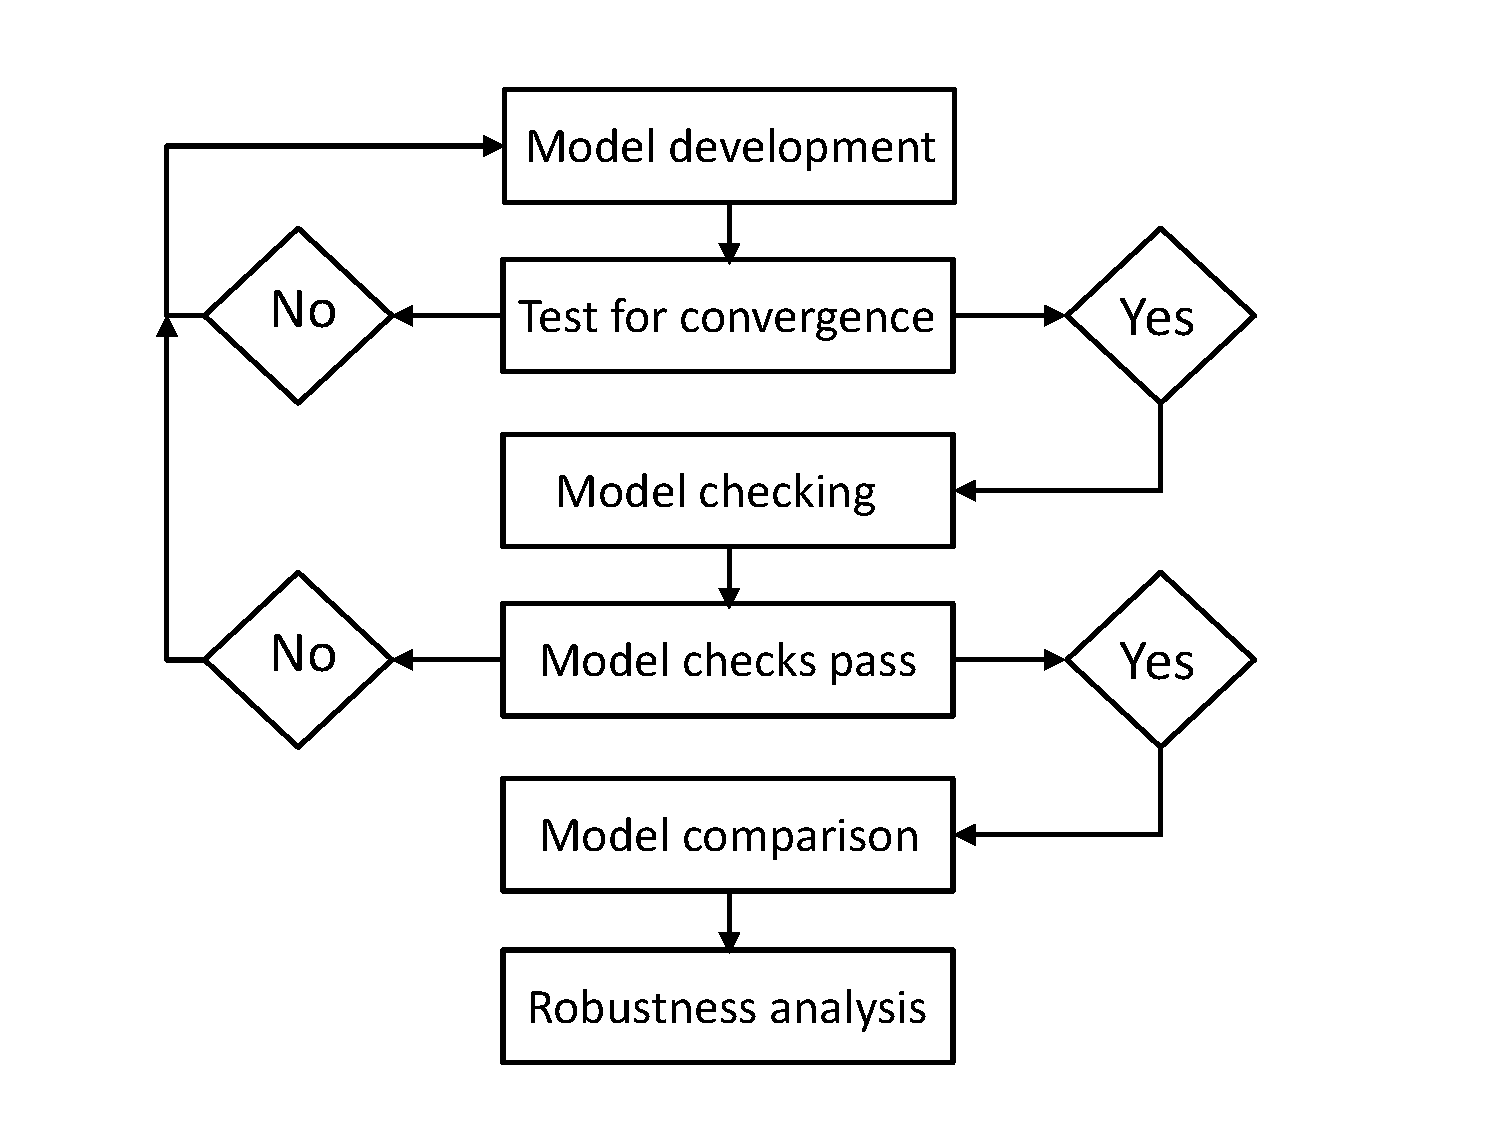
\includegraphics[width=170mm]{Bayesian_modeling_decision_diagram.pdf}
        \caption{} \label{fig:decision}
      \end{center}
    \end{figure*}

    \begin{figure*}
      \begin{center}
        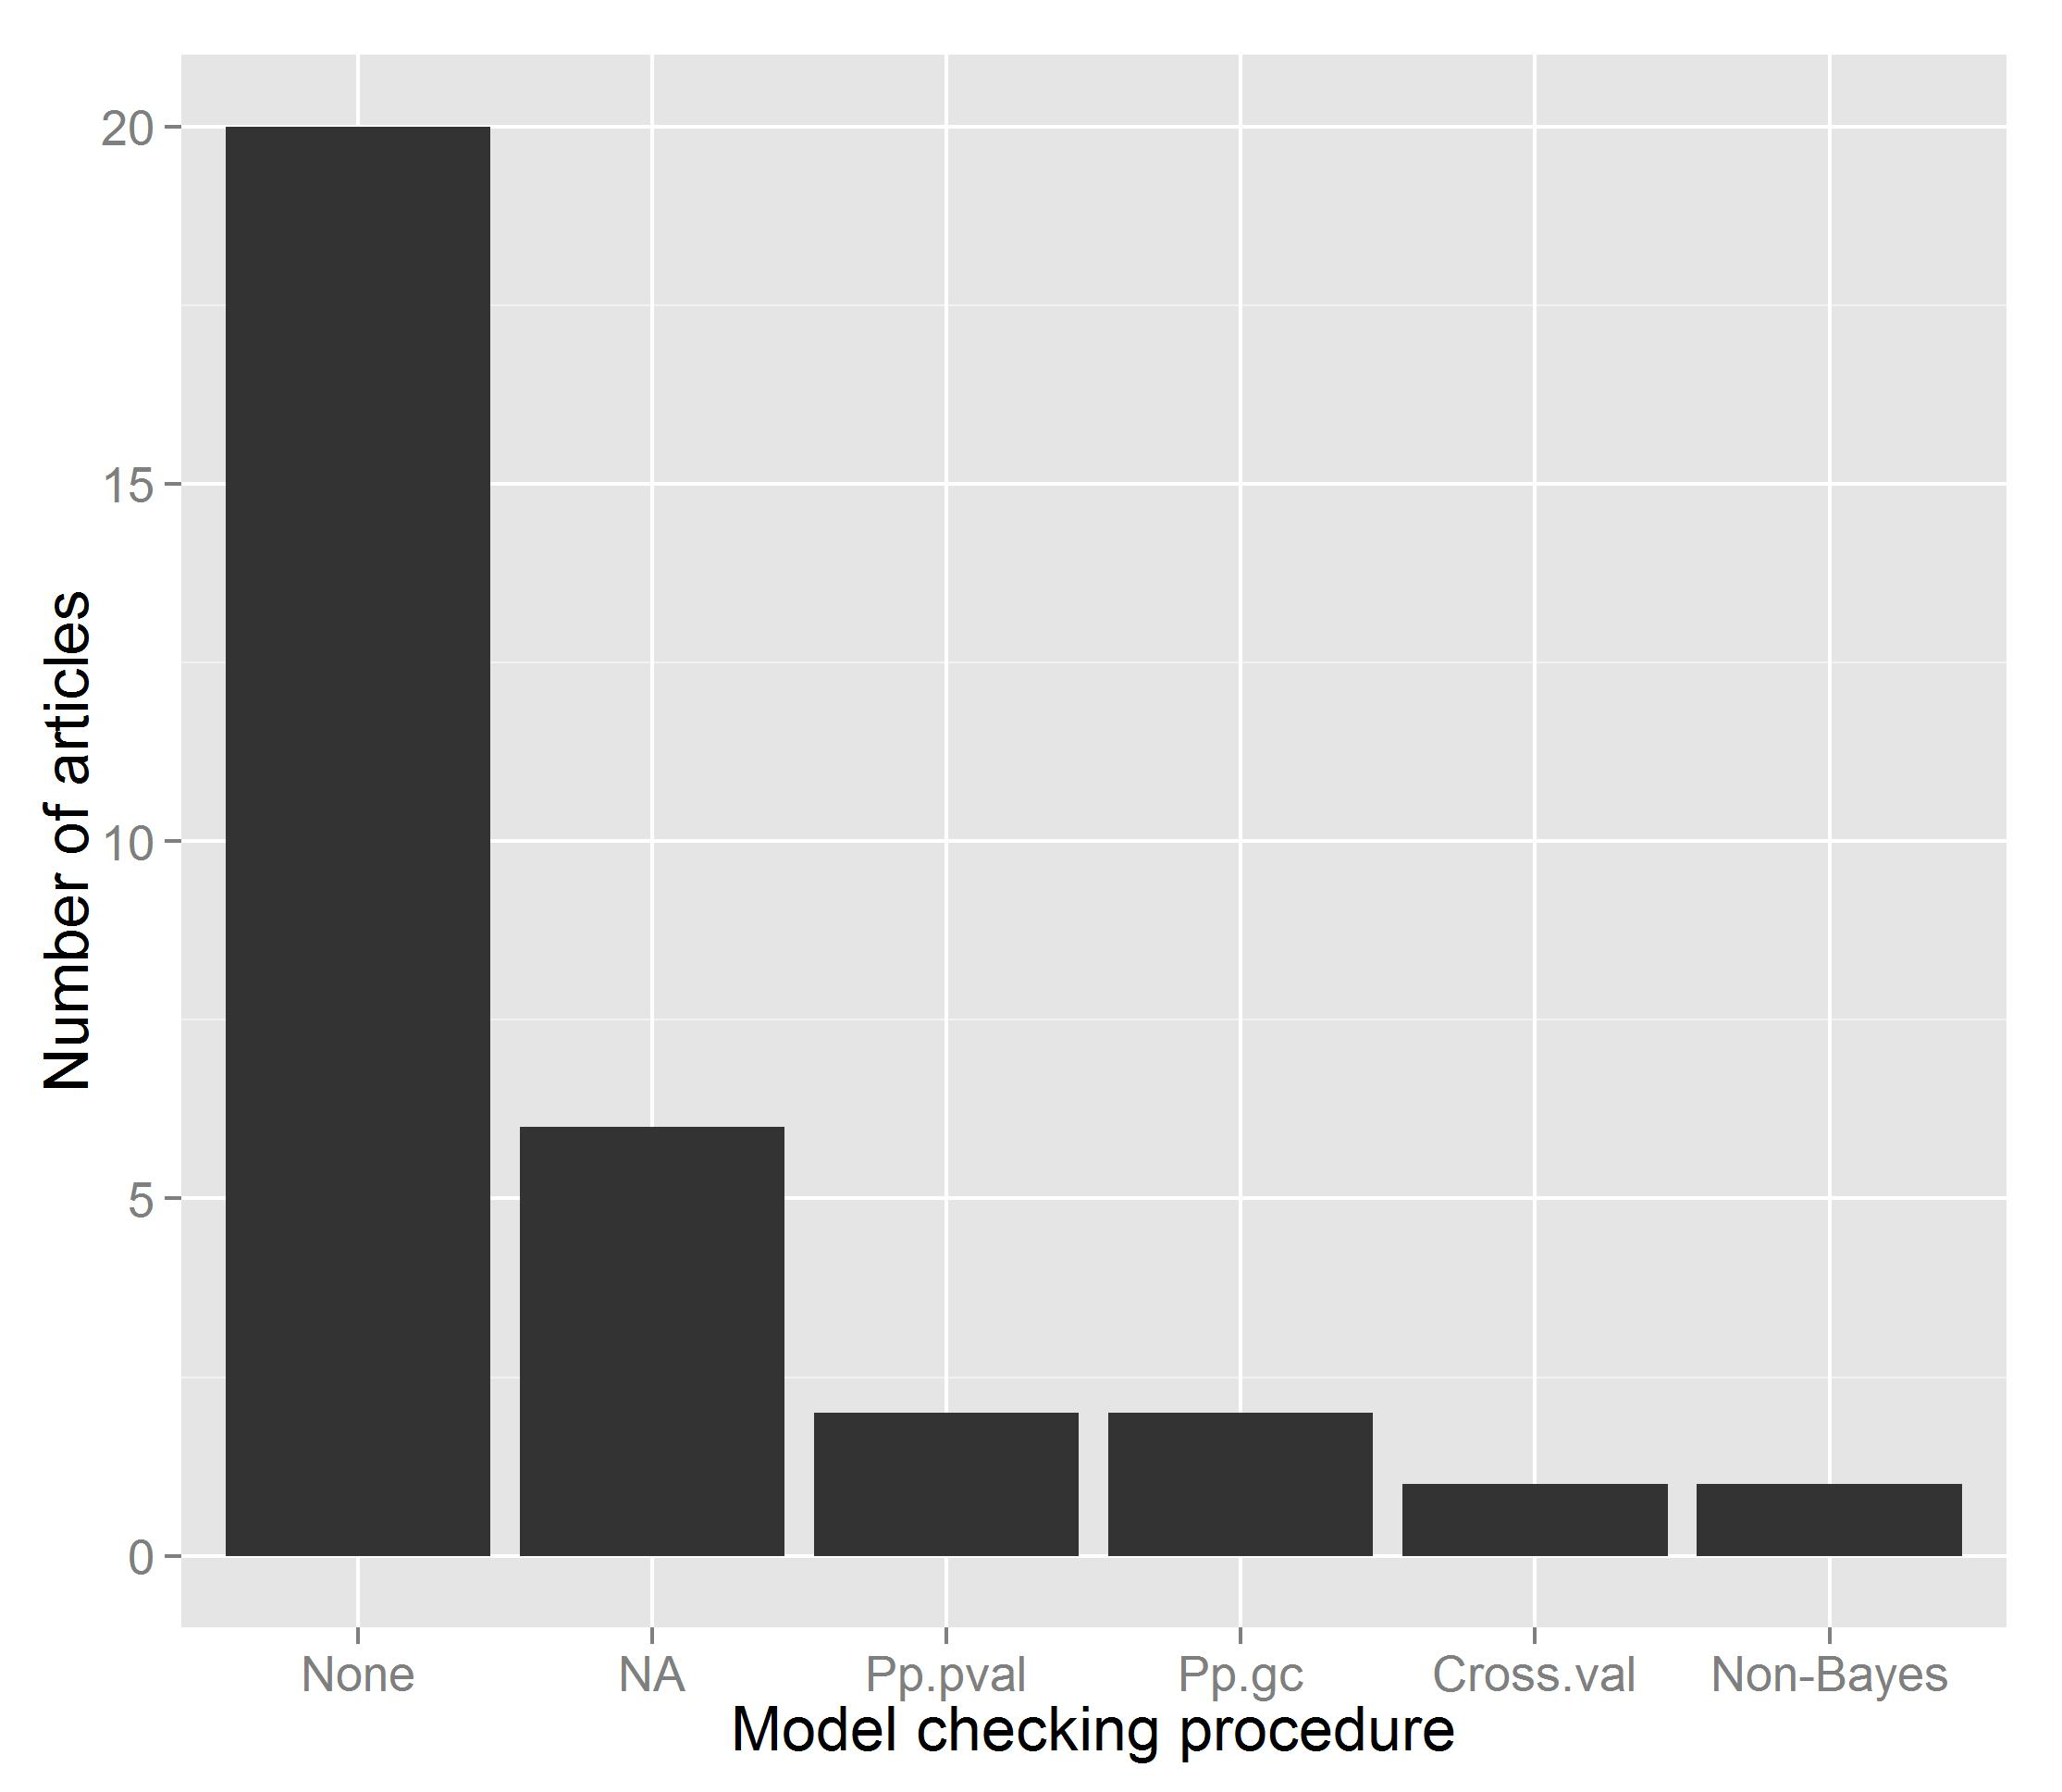
\includegraphics[width=170mm]{WOSsearch.jpeg}
        \caption{} \label{fig:WOS}
      \end{center}
    \end{figure*}

    \begin{figure*}
      \begin{center}
        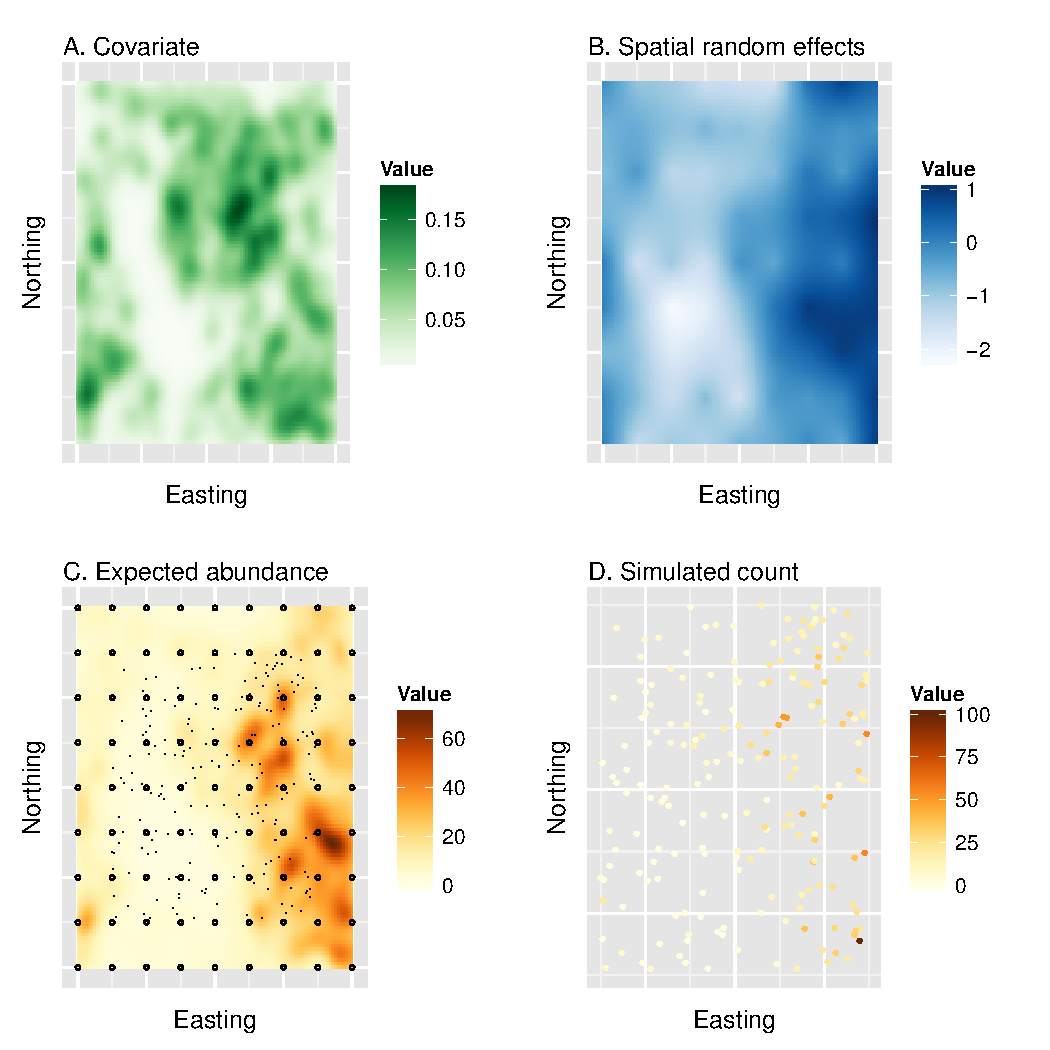
\includegraphics[width=170mm]{sim_count_maps.pdf}
        \caption{} \label{fig:sim_maps}
      \end{center}
    \end{figure*}

    \begin{figure*}
      \begin{center}
        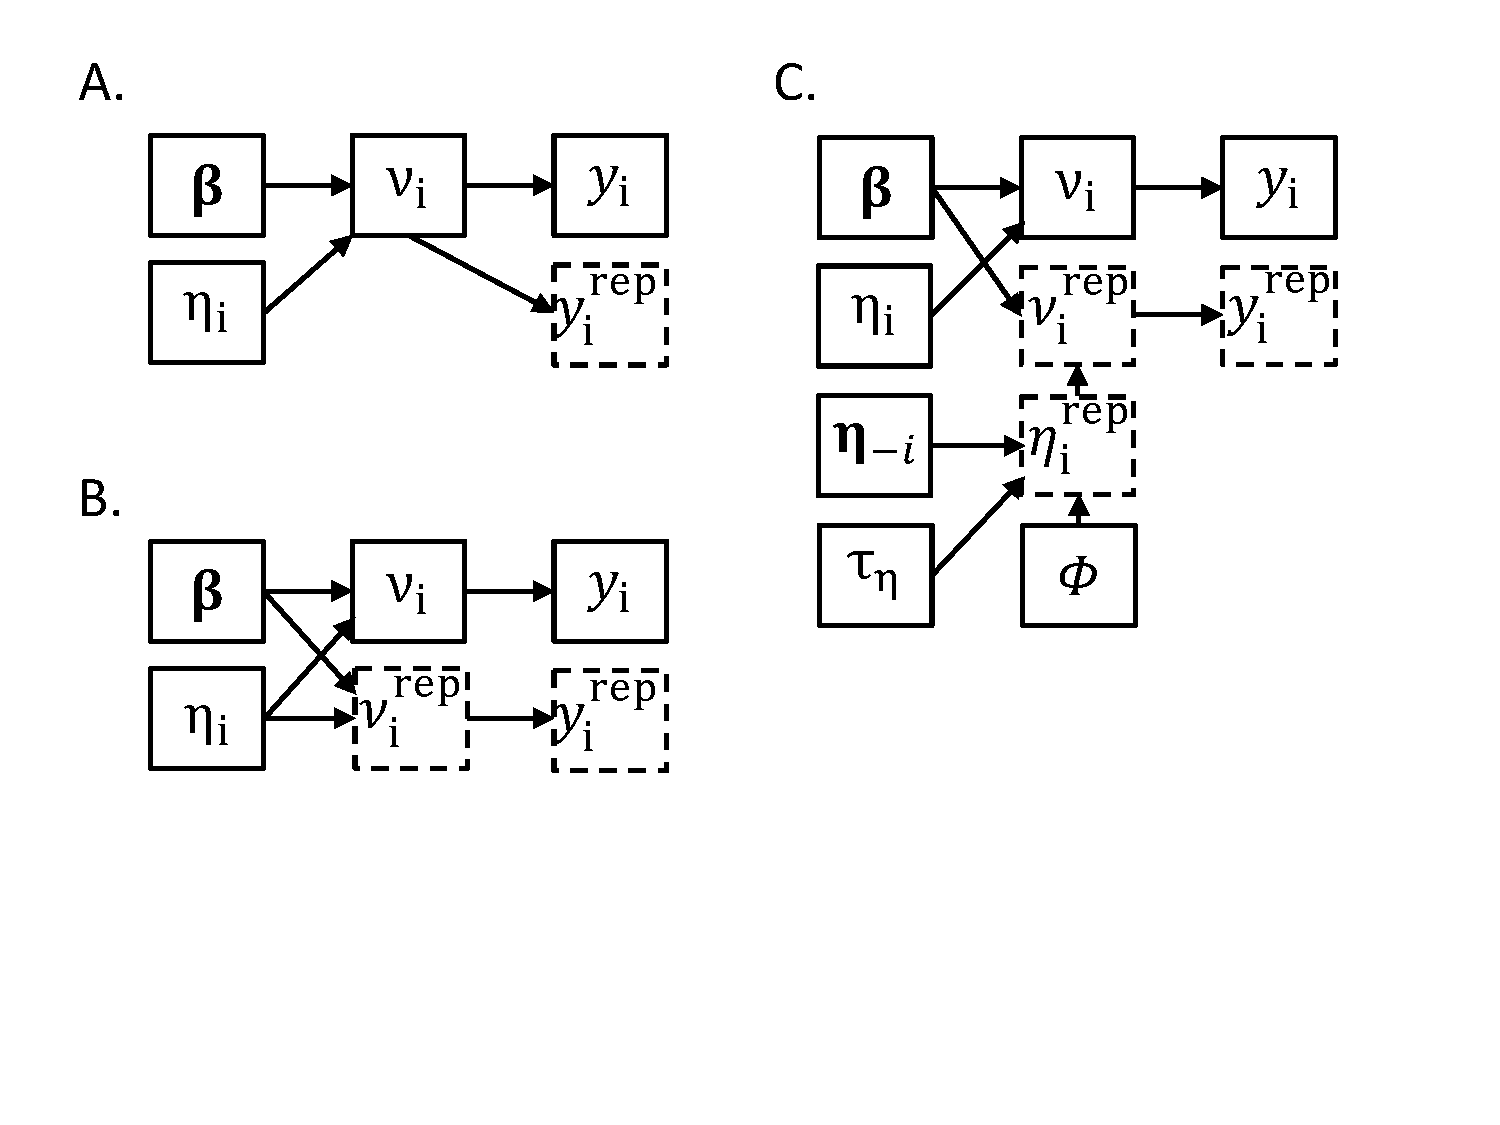
\includegraphics[width=170mm]{posterior_prediction_diagram.pdf}
        \caption{} \label{fig:post_pred}
      \end{center}
    \end{figure*}

    \begin{figure*}
      \begin{center}
        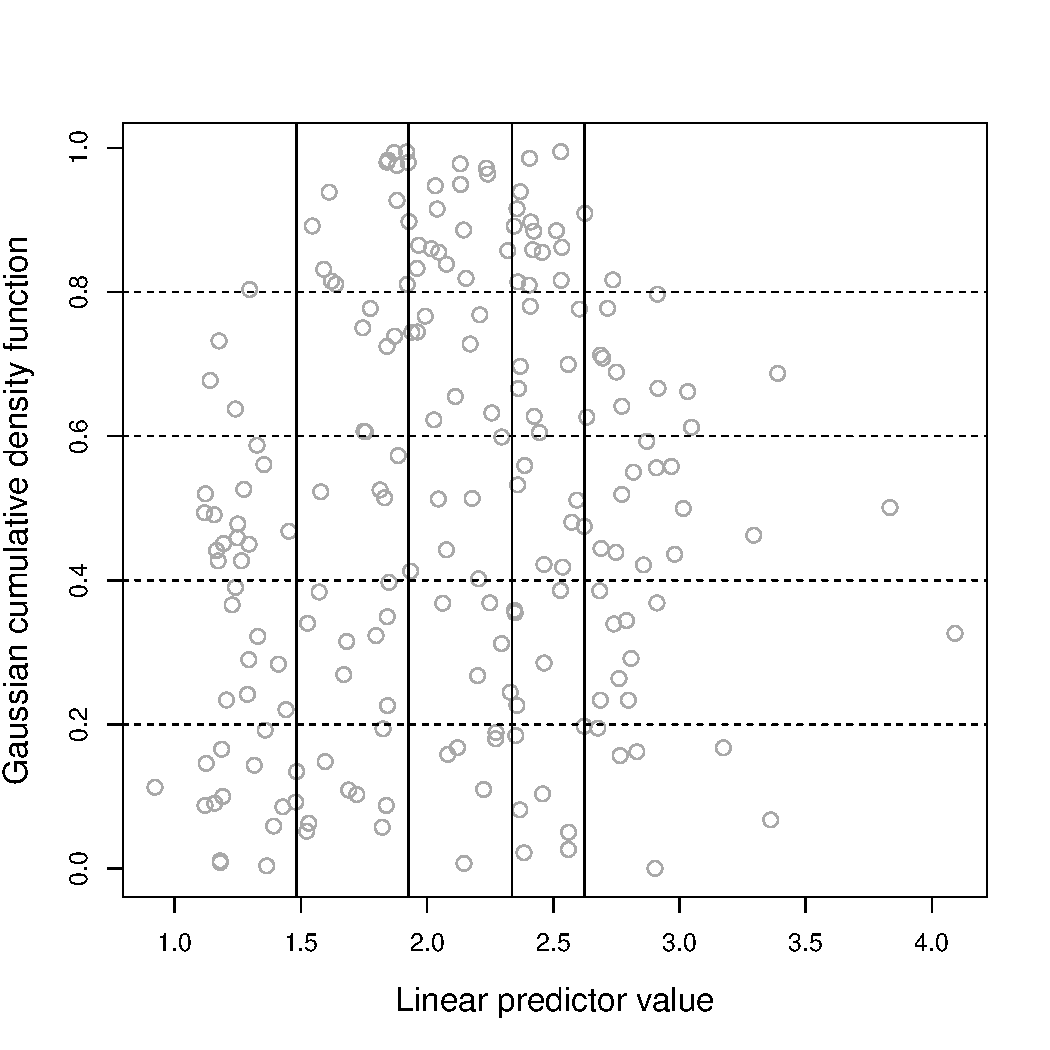
\includegraphics[width=170mm]{pivot_CDF_plot.pdf}
        \caption{} \label{fig:pivotCDF}
      \end{center}
    \end{figure*}

    \begin{figure*}
      \begin{center}
        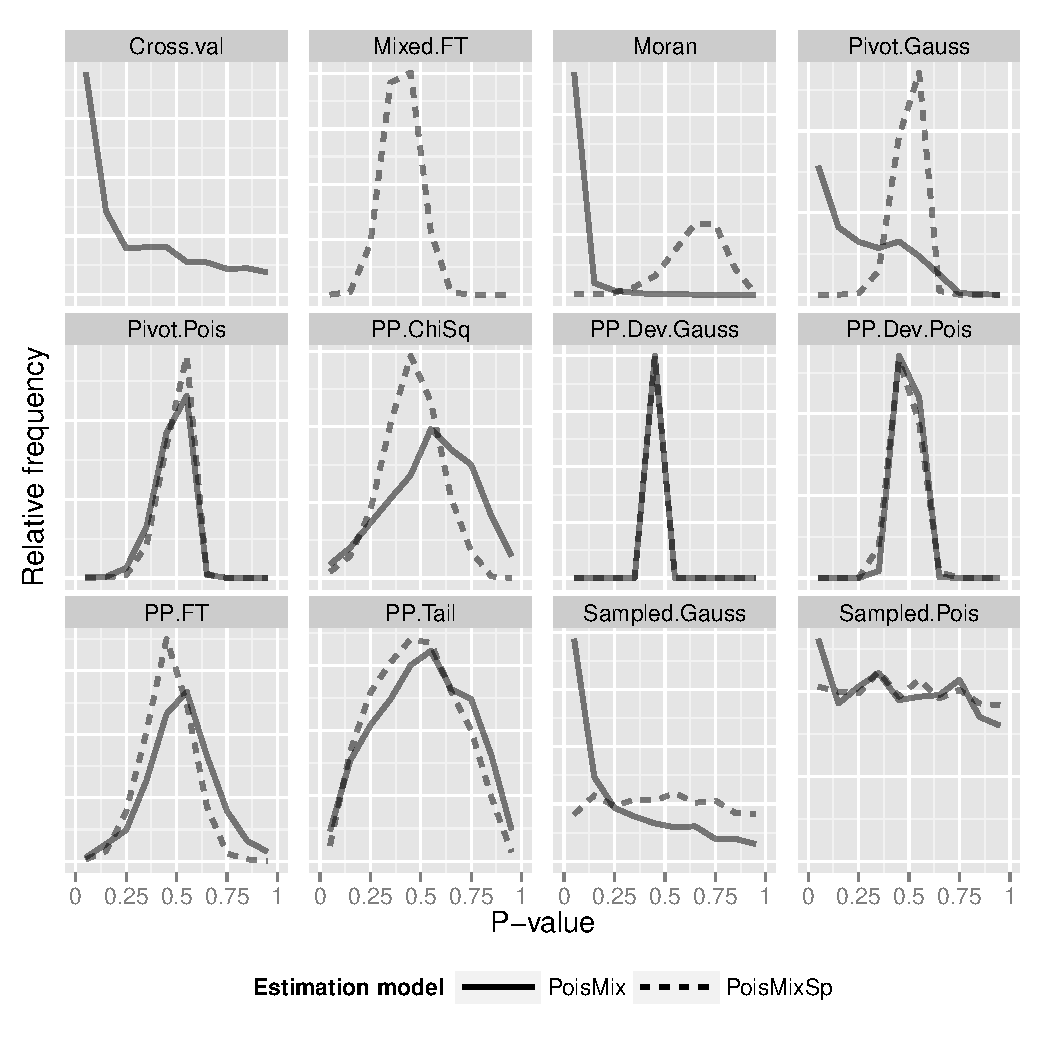
\includegraphics[width=170mm]{SpatRegSimPvals.pdf}
        \caption{} \label{fig:SpatReg_pvals}
      \end{center}
    \end{figure*}

    \begin{figure*}
      \begin{center}
        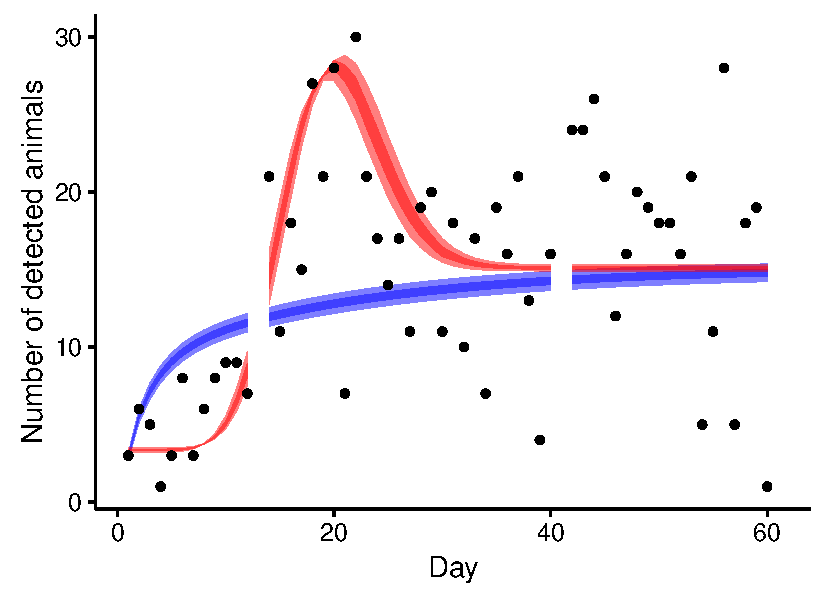
\includegraphics[width=170mm]{attendance_fit.pdf}
        \caption{} \label{fig:attend}
      \end{center}
    \end{figure*}


  \end{spacing}
\end{document}
